%%%%%%%%%%%%%%%%%%%%%%%%%%%%%%%%%%%%%%%%%%%%%%%%%%%%%%%%%%%%%%%%%%%%%%%%%%%

\documentclass[12pt]{report}

\usepackage{pslatex}
\usepackage[T1]{fontenc}
\usepackage[latin1]{inputenc}
\usepackage{geometry}
\geometry{letterpaper,pdftex,
          top=1.25in,
          footskip=0.75in,
          bottom=1.25in,
          left=1.25in,
          right=1.25in}
\usepackage{setspace}
\usepackage{verbatim}
\usepackage{mdwlist}
\usepackage{multirow}

\usepackage{graphicx}

\IfFileExists{url.sty}{\usepackage{url}}
                      {\newcommand{\url}{\texttt}}

\usepackage{hyperref}
\hypersetup{%
    pdfborder = {0 0 0}
}

\usepackage[labelfont=bf]{caption}

%\makeatletter
%\usepackage{babel}
%\makeatother

\usepackage{fixltx2e}
%%\usepackage{flafter}

\usepackage{fancybox}
\usepackage{fancyvrb}
\VerbatimFootnotes
% 1.5 = par indent, 2.5 = block quote indent
\newenvironment{code}
  {\Verbatim[xleftmargin=0.8em,fontsize=\small,baselinestretch=1.0,samepage=true]}
%  {\endVerbatim}
  {\endVerbatim\vspace{-2.6pt plus -0.87pt minus -0.87pt}}
%  {\endVerbatim\vspace{-2.5pt plus -0.83pt minus -0.83pt}}
\DefineVerbatimEnvironment
  {code*}{Verbatim}{fontsize=\small,baselinestretch=1.0,samepage=true}
\newenvironment{codef}
  {\Verbatim[fontsize=\small,baselinestretch=1.0]}
  {\endVerbatim\vspace{-\medskipamount}}
\newenvironment{codefnum}
 {\Verbatim[fontsize=\small,baselinestretch=1.0,numbers=left,numbersep=6pt]}
 {\endVerbatim\vspace{-\smallskipamount}}
\CustomVerbatimCommand{\sverb}{Verb}{fontsize=\small}
%\usepackage{listings}
%\lstset{basicstyle=\ttfamily\small,language={}}

\newcommand{\ID}{{\tt\it ID}}
\newcommand{\VALUE}{{\tt\it VALUE}}
\newcommand{\FLAG}{{\tt\it FLAG}}

\newcommand{\FIXME}[1]{[\textbf{FIXME}: \textit{#1}]}
\newcommand{\FIXMEQ}[1]{[\textbf{FIXME?}: \textit{#1}]}
\newcommand{\HELP}[1]{[\textbf{HELP}: \textit{#1}]}
\newcommand{\FIXMEf}[1]{\footnote{\textbf{FIXME}: #1}}
\newcommand{\FIXMEQf}[1]{\footnote{\textbf{FIXME?}: #1}}
\newcommand{\NOTE}[1]{[\textbf{NOTE}: \textit{#1}]}
%newcommand{\fixme}[1]{[\textbf{FIXME}: \textit{#1}]}
%newcommand{\fixmeq}[1]{[\textbf{FIXME?}: \textit{#1}]}
%newcommand{\fixmef}[1]{\footnote{\textbf{FIXME}: #1}}
%newcommand{\fixmeqf}[1]{\footnote{\textbf{FIXME?}: #1}}
\newcommand{\fixme}[1]{}
\newcommand{\fixmeq}[1]{}
\newcommand{\fixmef}[1]{}
\newcommand{\fixmeqf}[1]{}
%\newcommand{\NOTE}[1]{}
\newcommand{\mynote}[1]{}
%\newcommand{\comment}[1]{}

\newcommand{\snip}[1]{\texttt{#1}}
\DefineShortVerb{\|}

\newenvironment{apil}
  {\begin{list}{}{\leftmargin=0em\itemsep=\medskipamount\topsep=-\parskip}}
  {\end{list}}
\newenvironment{apill}
  {\begin{list}{}{\leftmargin=1em\itemsep=-\parsep\topsep=-\parskip}}
  {\end{list}}
\newcommand{\kw}[1]{\textbf{#1}}

\newenvironment{table-changes}
  {\begin{table}[h]}
  {\end{table}}

\sloppy

%%%%%%%%%%%%%%%%%%%%%%%%%%%%%%%%%%%%%%%%%%%%%%%%%%%%%%%%%%%%%%%%%%%%%%%%%%%

\hypersetup{
  pdftitle={ZL},
  pdfauthor={Kevin Atkinson}}

\newcommand{\theoverviewfig}{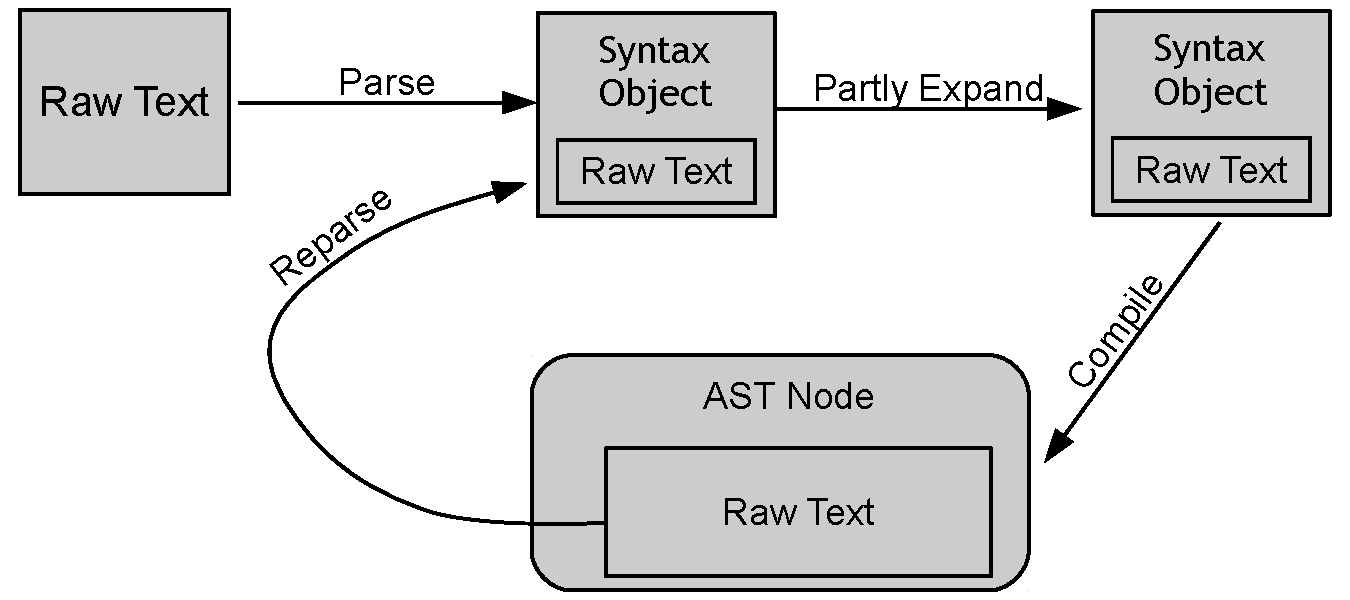
\includegraphics[width=4.5in]{parsing-overview}}
\newcommand{\thefig}{%\renewcommand{\arraystretch}{1.0}
{
\small
\setlength{\fboxsep}{0pt}
\cornersize*{10pt}

\newenvironment{rawtext}[1]
  {\begin{tabular}{|l|}\hline\begin{minipage}{#1}}
  {\end{minipage}\\\hline\end{tabular}}
\newenvironment{syntax}[1]
  {\begin{tabular}{|l|}\hline\begin{minipage}{#1}}
  {\end{minipage}\\\hline\end{tabular}}
\newenvironment{flow}
  {\begin{tabular}{c}
   \\[-8pt]}
  {\\[-8pt] \\
   \end{tabular}}
\newenvironment{compiled}[1]{%
\begin{Sbox}
\begin{tabular}{#1}
}{%
\end{tabular}
\end{Sbox} 
\ovalbox{\TheSbox \hspace*{-2.5pt}}
}

\DefineVerbatimEnvironment
  {figcode}{Verbatim}{fontsize=\small,baselinestretch=1.0,samepage=true}

\newcommand{\thrule}{\rule{0pt}{9.5pt}}

\newcommand{\transf}[1]{\rule[-3pt]{0pt}{12pt}$\downarrow$#1$\downarrow$}

\newcommand{\Ol}{4.8in}
\newcommand{\Il}{4.3in}
\newcommand{\IIl}{3.5in}
\newcommand{\IIIl}{3in}

%\setlength{\fboxsep}{0pt}

%\newcommand{\Ol}{3in}
%\newcommand{\Il}{2.75in}
%\newcommand{\IIl}{2.5in}
%\newcommand{\IIIl}{2.25in}

\begin{flow}
  \begin{rawtext}{\Ol}
  \begin{figcode}
inline int f() {int x = 10; return x;}
int main() {return f();}
  \end{figcode}
  \end{rawtext}
  \\
  \transf{PARSE}
  \\
  \begin{syntax}{\Ol}
  \begin{figcode}
(@ (stmt inline int f ("()" "") ("{}" "int x = 10; return x;")
   (stmt int main ("()" "") ("{}" "return f();")))
  \end{figcode}
  \end{syntax}
  \\
  \transf{EXPAND \& COMPILE}
  \\
  \begin{compiled}{l}
  \thrule \textit{TOP-LEVEL ENVIRONMENT}\\
  \hline
    \begin{flow}
      \begin{syntax}{\Il}
      \begin{figcode}
(stmt inline int f ...)
      \end{figcode}
      \end{syntax}
      \\
      \transf{EXPAND}
      \\
      \begin{syntax}{\Il}
      \begin{figcode}
(fun f "()" int :inline ("{}" "int x = 10; return x;"})
      \end{figcode}
      \end{syntax}
      \\
      \transf{COMPILE}
      \\
      \begin{compiled}{l|l}
        \multicolumn{2}{l}{\thrule FUN} \\
        \hline
        inline & \textit{true} \\
        \hline
        id & f \\
        \hline
        type & int \\
        \hline
        body & \begin{flow}
          \begin{syntax}{\IIl}
          \begin{figcode}
("{}" "int x = 10; return x;")
          \end{figcode}
          \end{syntax}
          \\
          \transf{EXPAND \& REPARSE}
          \\
          \begin{syntax}{\IIl}
          \begin{figcode}
(block (stmt int x = 10)
       (return (exp x)))
          \end{figcode}
          \end{syntax}
          \\
          \transf{COMPILE}
          \\
          \begin{compiled}{l}
            \thrule BLOCK\\
            \hline
            \begin{flow}
              \begin{syntax}{\IIIl}
              \begin{figcode}
(stmt int x = 10))
              \end{figcode}
              \end{syntax}
              \\
              \transf{EXPAND}
              \\
              \begin{syntax}{\IIIl}
              \begin{figcode}
(var x (int) (exp 10))
              \end{figcode}
              \end{syntax}
              \\
              \transf{COMPILE}
              \\
              \begin{compiled}{l}
                \thrule VAR \\
                \hline
                ... \\
              \end{compiled}
            \end{flow} \\
            \hline
            \begin{flow}
              \begin{syntax}{\IIIl}
              \begin{figcode}
(return (exp x))
              \end{figcode}
              \end{syntax}
              \\
              \transf{...}
            \end{flow} \\
          \end{compiled}
        \end{flow}\\
      \end{compiled}
    \end{flow}
    \\
    \hline
    \begin{flow}
      \begin{syntax}{\Il}
      \begin{figcode}
(stmt int main ...)
      \end{figcode}
      \end{syntax}
      \\
      \transf{...}
    \end{flow}
    \\
  \end{compiled}
  \\
\end{flow}
}
}

\begin{document}

\pagenumbering{roman}


\begin{titlepage}
\begin{center}
\vspace*{\fill}
{\huge ZL\\[0.5em]}
{\large \it (\href{http://zl-lang.org}{zl-lang.org})}\\[\fill]
{\large Kevin Atkinson}\\[\fill]
{\Large \textsc{Draft}\\[0.5em]}
{\large \today}\\[\fill]
Copyright \copyright\ Kevin Atkinson\ 2011--2012\\
GNU LGPL 2.1 or later
\end{center}
\end{titlepage}

\pagebreak
\setcounter{page}{2}

\begingroup
\onehalfspacing

%% Used to check spacing around code blcoks
%\noindent
%XXXXXXXXXXXXXXXXXXXXXXXXXXXXXXX
%\begin{code}
%XXXXXXXXXXXXXXXXXXXXXXXXX
%\end{code}
%XXXXXXXXXXXXXXXXXXXXXXXXXXXXXXX

%\chapter*{Abstract}
%\input{abstract}

\chapter*{Copyright and Acknowledgment}

This documentation is under the same license of ZL itself; you can
redistribute and/or modify both this documentaion and ZL itself under
the terms of the GNU Lesser General Public License as published by the
Free Software Foundation; either version 2.1 of the License, or (at
your option) any later version.  You should have received a copy of
the GNU Lesser General Public License along with this documentaion; if
not, write to the Free Software Foundation, Inc., 51 Franklin Street,
Fifth Floor, Boston, MA 02110-1301 USA or see
\url{http://www.gnu.org/licenses/lgpl-2.1.html}.


This documentation was originally based on the first author's
Dissertation~\cite{abi-diss}.  The disseration is based on an earlier
work~\cite{abi-gpce10}: ``ABI Compatibility Through a Customizable
Language'', Proceedings of the
\textit{Ninth International Conference on Generative Programming and
  Component Engineering (GPCE'10)}, Eindhoven, The Netherlands,
Oct. 2010. \copyright\ ACM, 2010,
\url{http://dx.doi.org/10.1145/1868294.1868316}, of which Matthew Flatt 
and Gary Lindstrom are co-authors.  Parts of the dissertation also
appeared in the work~\cite{zl-scheme11}: ``Adapting Scheme-Like Macros
to a C-Like Language'', \textit{Workshop on Scheme and Functional
Programming}, Portland, Oregon, Oct. 2011, of which Matthew Flatt is a
co-author.


\endgroup

\tableofcontents
%\listoffigures
%\listoftables

\pagebreak
\setcounter{page}{1}
\pagenumbering{arabic}

\begingroup
\onehalfspacing

%%%%%%%%%%%%%%%%%%%%%%%%%%%%%%%%%%%%%%%%%%%%%%%%%%%%%%%%%%%%%%%%%%%%%%%%%%%%%
\chapter{Introduction}
\label{intro}

C is a simple language that gives the user considerable control
over how source code maps to machine code.  For example, structures are
guaranteed to be laid out in a particular way, dynamic memory is not
allocated unless it is asked for, all function calls are explicit, and
the only functions created are the ones that are explicitly defined.
For this reason, most low-level system code is written in C.  Nevertheless
programmers want to use high-level language constructs for various
reasons, and such use generally relinquishes low-level control.
For example, C++ does not guarantee a particular layout of objects.
This lack of control can cause a number of problems, including
compatibility problems between different releases of software and
between different compilers.

A programmer can regain control over higher-level language feature
implementation through an extensible compiler.  To provide such
extensibility, macros for C are an ideal choice.  Macros for C let a
programmer build higher-level constructs from a small core, rather
than forcing a programmer to accept a built-in
implementation. Moreover, since macros elevate language extensions to
the level of a library, individual advanced language features are only
active when loaded.

A simple macro system, such as the C preprocessor, is not adequate for
this purpose, nor is any macro system that acts simply as a
preprocessor.  Rather, the macro system must be an integral part of
the language that can do more than rearrange syntax.  In addition, the
C base language must be extended to support the necessary primitives
for implementing higher-level features.  ZL, a new C-compatible and
C++-like systems programming language in development, addresses both
of these needs.

This document presents ZL.  Chapter \ref{zl-tutorial} gives an into of
ZL features in the form of a tutorial.  The other chapters give a
detail overview of ZL features.  The appendices give information on
some of ZL's implementation.

The document is a work in progress.  Proofreading of this document is
greatly appreciated.  The easiest thing is to just edit the source
(please, no reformatting!) and submit a pull request with
your corrections.

%% ZL Goals:

%% \begin{itemize}
%% \item Customizable
%% \item Control
%% \end{itemize}

%%%%%%%%%%%%%%%%%%%%%%%%%%%%%%%%%%%%%%%%%%%%%%%%%%%%%%%%%%%%%%%%%%%%%%%%%%%%%%
\chapter{ZL Tutorial}
\label{zl-tutorial}

This chapter will give you an overview of ZL with a focus on ZL
extensibility features.

\section{Hello World}

ZL basic syntax is the same as it is in C or C++ therefor a simple
Hello World program is nothing but:

\begin{code}
int main() {
  printf("Hello World!")
}
\end{code}

To compile, save this file to |hello.zl| and then use zlc:
\begin{code}
zlc hello.zl
\end{code}
which should create an excitable |a.out| which you can run.

Note that there is no |#include| line in the source file.  The ZL
prelude includes some of the more common functions from the C standard
library and ZL source files are not run through the C preprocessor
by default.

The driver script |zlc| is meant to act as a drop drop in replacement
for GCC.  For example,
\begin{code}
zlc main.zl file1.cpp file2.zlp -o main
\end{code}
compiles the pure ZL source file |main.zl|, the C++ source file
|file1.cpp|, and the ZL source file |file2.zlp| into an executable
|main|.  Each file is compiled slightly differently based on the
extension as ZL has different modes for C, C++, and ZL source files.
In addition C, C++, and ZL source files with the |.zlp| extension are
run through the C preprocessor to handle includes and other
token-level macros that the higher-level ZL macro processor can not
handle.  As already mentioned, pure ZL files with |.zl| extension are
not preprocessed.

\section{Macro Introduction: A Perl Like Or}
\label{pattern-macros}

C's or operator returns a boolean value.  Sometimes it would be more
convenient if it returns the first true value like Perl does.  For
example if we wanted to use the first non-NULL pointer we could use:
\begin{code}
some_call(or(p1,p2))
\end{code}
where |p1| and |p2| are pointers.  Defining |or| as a function (or even
a function template) will not work because the |or| macro should not
evaluate the second argument if the first one evaluates to a true
value.

Fortunately, ZL makes it very easy to define simple macros such as this
using the |macro| form:
\label{or}
\begin{code}
macro or(x, y) { ({typeof(x) t = x; t ? t : y;}); }
\end{code}
(In ZL, as in GCC, the |({...})| is a statement expression whose value
is the result of the last expression, and |typeof(x)| gets the type of
a variable.)  Like Scheme macros~\cite{syn-abst}, ZL macros
are hygienic, which means that they respect lexical scope.  For
example, the |t| used in |or(0.0, t)| and the |t| introduced by the
|or| macro remain separate, even though they have the same symbol
name.

\paragraph{Syntax Macros.}

It is even possible to locally redefine the behavior of the built-in
\verb/||/ operator so that we could instead just use \verb/p1 || p2/.
All that is required to archive this transformation is to change the
|macro| to |smacro|:
\begin{code}
smacro or(x, y) { ({typeof(x) t = x; t ? t : y;}); }
\end{code}
The |smacro| form defines a \textit{syntax macro} which operates on
syntax, as oppose to the |macro| form which defines a \textit{function-call
  macro} in which calls to it take the shape of a function call.

The syntax version of the |or| macro works because ZL performs most of
its operations using interment S-expression like language.  For
example \verb/p1 || p2/ is parsed as |(or p1 p2)|, before being
converted into an AST (details of which are given in Chapter
\ref{parsing})

\paragraph{Keyword Parameters.}

The |or| macro above has too \textit{positional} parameters.  Macros
can also have \textit{keyword} parameters and \textit{default values}.
For example:
\begin{code}
macro sort(list, :compar = strcmp) {...}
\end{code}
defines the macro |sort|, which takes the keyword argument |compar|,
with a default value of |strcmp|.  A call to sort will look something
like {\tt|sort(list,| |:compar = mycmp)|}.

\section{Classes and Templates}
\label{template-intro}

ZL also supports a limited subset of C++ which includes classes and
very basic template support.  Classes are defined if the usual way.  ZL
recognizes the template syntax, but templates are defined using a
macro and must be explicitly instantiated by calling the macro.  For
example, to use a |vector| of type |int|:

\begin{code}
mk_vector(int)

int main() {
  vector<int> con;
}
\end{code}

We will revisit the |mk_vector| macro in Section \ref{mk_vector}.

\section{Extending The Grammar: Foreach}
\label{foreach}

One very common operation is to iterate through the elements of a
container.  It is such a common operation that support for it was
incorporated latest version of the C++ standard via special version of
the |for| loop.  ZL doesn't support this version, but we can very
easily define a similar construct.  Instead of extending the syntax of
|for| we will define a new syntax form: |foreach|.  The usage of the
form is straightforward; for example, the following code prints all the
elements of a vector:
\begin{code}
int main() {
  vector<int> con;
  ...
  foreach (elm in con) {
    printf("%d\n");
  }
}
\end{code}

The first thing we need to do to support the new |foreach| form is to
define some new syntax.  ZL provides basic support for new syntax by
extending the PEG using the |new_syntax| form.  We add support the new
loop form by rewriting the |CUSTOM_STMT| production as follows:
\begin{code}
new_syntax {
  CUSTOM_STMT := _cur / <foreach> "foreach" "(" {ID} "in" {EXP} ")" {STMT};
}
\end{code}
The special |_cur| production refers to the previous version of the
|CUSTOM_STMT| and anything between |{}| becomes a subpart of the
syntax object that is named between the |<>|. 
With the new syntax defined the definition of the macro is fairly
straightforward:

\begin{code}
smacro foreach (VAR, WHAT, BODY) {
  typeof(WHAT) & what = WHAT;
  typeof(what.begin()) i=what.begin(), e=what.end();
  for (; i != e; ++i) {
    typeof(*i) & VAR = *i;
    BODY;
  }
}
\end{code}

Chapter \ref{parsing} gives more details on the PEG and how to
extend it.

\section{Procedural Macros}
\label{foreach-proc}

All the macros shows so far are simple \textit{pattern-based} macros.
Sometimes we need to do more than simply rearrange syntax.  For
example, in the |foreach| macro of the previous section, if the
container lacks a |begin| or |end| method ZL will return a cryptic
error message which will refer to the expanded output, rather than the
user input; it would be far better to give a straightforward error
message which refers to the user input.  For these more complex tasks
ZL provides support for procedural macros which can take action base on
their input.

A procedural macro is a function which maps one syntax object to
another.  ZL provides special syntax support for defending these
functions.  They look a lot like pattern-based macros expect that the
keyword |proc| proceeds the macro and the body of the macro is ZL code
rather than the expanded output.  Syntax is created using special
quasiquote syntax.  For example, the following macro defines a
version of the |foreach| which returns an error message if the
container lacks the proper methods:
\begin{code}
proc smacro foreach (VAR, WHAT, BODY) {
  Syntax * what = ``WHAT;
  if (!symbol_exists(``begin, what) || !symbol_exists(``end, what))
    return error(what, "Container lacks begin or end method.");
  return `{
    typeof(WHAT) & what = WHAT;
    typeof(what.begin()) i=what.begin(), e=what.end();
    for (;i != e; ++i) {typeof(*i) & VAR = *i; BODY;}
  };
}
\end{code}

The |symbol_exists| and |error| are API functions which are callbacks
into the compiler.  The \verb/``/ and \verb/`{/ are quasiquotes; the
first forms quotes an identifier; the second form quotes arbitrary
syntax.  Pattern variables can only be used inside quasiquotes;
however, the |symbol_exists| and |error| function requires a syntax
object.  Hence, \verb/``WHAT/ is used to extract the syntax object
associated with the pattern variable and store it in a local variable.

\paragraph{Antiquotes.}

Rather than using pattern variables, it is possible to use antiquotes
to store the result of the match in local variables by prefixing the
variable with a \verb/$/.  For example, here is a version of foreach
that uses antiquotes instead:
\begin{code}
proc smacro foreach ($var, $what, $body) {
  if (!symbol_exists(``begin, what) || !symbol_exists(``end, what))
    return error(what, "Container lacks begin or end method.");
  return `{
    typeof($what) & what = $what;
    typeof(what.begin()) i=what.begin(), e=what.end();
    for (;i != e; ++i) {typeof(*i) & $var = *i; $body;}
  };
}
\end{code}

When an antiquote is used when matching syntax the results of the
match are stored in a local variable hence \verb/$body/ gets stored in
the local variable |body|, which is then used for by the
|symbol_exist| and |error| function.  When an antiquote is used inside
quasiquotes than it is replaced with the value of the expression; in
most cases this is a local variable.

\paragraph{Additional Info.}

Shown here is only a small taste of what procedural macros can do.  ZL
procedural macros are very powerful and in many ways, act more as
an extension to the compiler than a simple macro that transforms text
from one form to another.  Chapter \ref{proc-macros} gives additional
information on procedural macros, which includes a lower level and
more powerful API.

\section{Templates and Bending Hygiene}
\label{mk_vector}

As already mentioned in Section \ref{template-intro}, ZL does not have builtin
template support.  Instead a macro can be used to create instances of
a template.  Figure \ref{vector-impl} shows the macro and supporting
code to create for the |vector| template class.
\begin{figure}
\begin{codef}
template vector;

macro mk_vector (T,@_) :(*)
{
  __once vector<T>
  class vector<T> {
  private:
    T * data_;
    T * end_;
    T * storage_end_;
  public:
    typedef T * iterator;
    typedef const T * const_iterator;
    typedef size_t size_type;

    iterator begin() const {return data_;}
    iterator end()   const {return end_;}
    bool empty() const {return data_ == end_;}
    size_t size() const {return end_ - data_;}
    size_t max_size() const {return (size_t)-1;}
    size_t capacity() const {return storage_end_ - data_;}
    T & front() const {return *data_;}
    T & back() const {return *(end_-1);}
    T & operator[](size_t n) const {return data_[n];}
    vector<T>() : data_(NULL), end_(NULL), storage_end_(NULL) {}
    vector<T>(size_t n) : ... {resize(n);}
    vector<T>(const vector<T> & other) : ... {...}
    void push_back(const T & el) {...}
    void pop_back() {...}
    void assign(const T * d, unsigned sz) {...}
    void resize(size_t sz) {...}
    void erase(T * pos) {...}
    ~vector<T>() {...}
    ...
  };
}
\end{codef}
\caption{ZL implementation of vector template class}
\label{vector-impl}
\end{figure}

There are two things to note about this macro, the first is some
special syntax to make the template instance to behave as expected,
and the second is to bend normal hygiene rules so that |vector| and the
members of the class are visible outside the macro.

\paragraph{Special Template Syntax.}

Template classes have special syntax that ZL needs to know to
recognize; which is done using the |template| form (which is used
differently than it is in C++).  In addition templates have special
linkage rules so that there are not multiple instances of the same
template in the executable, hence |__once| is used to declare that
duplicate symbols should be merged when linking.  Other than that, the
body of the |mk_vector| is the same as it would be for a template
class in ZL.

\paragraph{Bending Hygiene.}
\label{macro-export-intro}

Normal hygiene rules will normally prevent the |mk_vector| macro from
working as expected as all symbols created will only be visible to the
macro itself.  To fix this ZL macros supports special syntax,
the~|:(*)|, which will \textit{export} top-level symbols from the
macro (which includes the members of the vector class).  Details of
exactly what is exported and how are given in Section
\ref{macro-export}.

It is also possible to export specific symbols by specifying the symbol
name instead of~|*|, again see Section \ref{macro-export} for the details.

\section{Bending Hygiene Part 2: Fancy Loops}
\label{fluid-intro}

In the previous section we needed to make the macro introduced symbols
visible outside the context of the macro.  Sometimes it is necessary
to make symbols visible to the parameters of the macros.  For this
case, ZL provides a different mechanism, the \textit{fluid binding}.
For example, if we wanted to create a version of the for loop which
also supports a Perl style redo we might try
\begin{code}
macro redo() {goto redo;}

smacro for (INIT, TEST, INC, BODY) {
  for (INIT; TEST; INC) {
    redo():
    BODY;
  }
}
\end{code}
(where the |for| used in the macro will refer to the builtin |for| and
not the macro itself and |redo:| is a label for the goto in the |redo|
macro).  A simple usage of the macro could be:

\begin{code}
int main() {
  for (int i = 0; i < 10; ++i) {
    ++i;
    printf("%d\n", i);
    if (i % 3 == 0)
      redo();
  }
}
\end{code}

Unfortunately this will not work.  The problem is the |redo| label
introduced in the |for| macro is private to that macro.  Exporting the
label will not help, as the label used in the |redo| macro is still
lexically scoped.  The export syntax only has meaning to new binding
forms not existing ones, hence that form can't be used.  ZL does provide a
way to make both |redo| labels totally unhygienic (see Section
\ref{replace_context}), but that solution will not compose well \cite{syn-parm}.

What is really needed is something akin to dynamic scoping in the
hygiene system.  That is, for the |redo| label to be scoped based on
where it is used when expanded, rather than where it is written in the
macro definition.  This can be done by marking the |redo| symbol as
|fluid| using |fluid_label| at the top level and then using |fluid|
when defining the symbol in local scope.  For example, the following
will allow the above to compile:

\begin{code}
fluid_label redo;

macro redo() {goto redo;}

smacro for (INIT, TEST, INC, BODY) {
  for (INIT; TEST; INC) {
    fluid redo:
    BODY;
  }
}
\end{code}

The general form to declare fluid binding is |fluid_binding|, the
details of which are described in Section \ref{fluid}

\section{User Types}
\label{user-types-intro}

ZL does not have a built-in notion of classes, rather the type system
has what is known as a \textit{user type} of which classes are built
from using macros.  A user type has two parts: a type, generally a
|struct|, to hold the data for the class instance, and a collection of
symbols for manipulating the data.

The collection of symbols is a \textit{module}.  For example,
\begin{code}
module M { int x;
           int foo(); }
\end{code}
defines a module with two symbols.  Module symbols are used by either
importing them into the current namespace, or by using the
special syntax |M::x|, which accesses the |x| variable in the above
module.

A user type is created by using the |user_type| primitive, which
serves as the module associated with the user type.  A type for the
instance data is specified using |associate_type|.

As an example, the class\footnote{For simplicity, we leave off access
  control declarations and assume all members are public in this
  work when the distinction is unimportant.}
\begin{code}
class C { int i; 
          int f(int j) {return i + j;} };
\end{code}
roughly expands to:
\begin{code}
user_type C {
  struct Data {int i;};
  associate_type struct Data;
  macro i (:this ths = this) {...}
  macro f(j, :this ths = this) {f`internal(this, j);}
  int f`internal(...) {...}
}
\end{code}
which creates a user type |C| to represent a class |C|; the structural
type |Data| is used for the underlying storage.  The macro |i|
implements the |i| field, while the |f| macro implements the |f|
method by calling the function |f`internal| with |ths| as the first
parameter.  Additional details of how classes are implemented are
given in Chapter \ref{class-user-type}.

\chapter{Parsing and Expanding}
\label{parsing}

The macros shown so far have been fairly simply.  Writing more
sophisticated macros, such as those required to implement classes,
requires some knowledge of parsing and macro expansion in ZL.  This
chapter gives the necessary background material, while the next
chapter details how to write such macros.

\section{Parsing Overview}
\label{parsing-overview}

To deal with C's idiosyncratic syntax while also allowing the syntax
to be extensible, ZL does not parse a program in a single pass.
Instead, it uses an iterative-deepening approach to parsing.  The
program is first separated into a list of partly parsed declarations
by a Packrat~\cite{peg-p,peg} parser that effectively groups
tokens at the level of declarations, statements, grouping curly
braces, and parentheses.  Each declaration is then parsed.  As it is
being parsed and macros are expanded, subparts, such as code between
grouping characters, are further separated.

ZL's iterative-deepening strategy is needed because ZL does not
initially know how to parse any part of the syntax involved with a
macro. When ZL encounters something that looks like a function call,
such as |f(x + 2, y)|, it does not know if it is a true function call
or a macro use.  If it is a macro use, the arguments could be
expressions, statements, or arbitrary syntax fragments, depending on
the context in which they appear in the expansion.  Similarly, ZL
cannot directly parse the body of a macro declaration, as it does not
know the context in which the macro will ultimately be used.

\pagebreak

More precisely, the ZL parsing process involves three intertwined
phases as shown in Figure \ref{parsing-overview-fig}. 
\begin{figure}
\begin{center}
\theoverviewfig
\end{center}
\caption{Overview of ZL's parsing process.}
\label{parsing-overview-fig}
\end{figure}
In the first phase \textit{raw text}, such as |(x+2)|, is 
parsed.  Raw text is converted into an intermediate form known as a
\textit{syntax object}, which can still have raw-text components.  
(Throughout this paper we show syntax objects as
S-expressions, such as |("()" "x+2")|.)  In the second phase, the
syntax object is expanded as necessary and transformed into other
syntax objects by expanding macros until a fixed point is reached.  In
the third phase, the fully expanded syntax object is compiled into an
\textit{AST}.

Figure \ref{fig} details ZL's parsing and expansion process.  
\begin{figure}
\begin{center}
\UndefineShortVerb{\|}
\thefig
\DefineShortVerb{\|}
\end{center}
\caption[How ZL compiles a simple program.]%
  {How ZL compiles a simple program.  The body of \texttt{f} is
   reparsed and expanded as it is being compiled.}
\label{fig}
\end{figure}
The top box contains a simple program as raw text, which is first parsed.
The result is a \textit{syntax list} (internally represented as a~|@|)
of |stmt|'s where each |stmt| is essentially a list of tokens, as
shown in the second box.  Each statement is then expanded and compiled
in turn, and is added to the top-level environment (which can be
thought of as an AST node). The third box in the figure shows how this
is done, which requires recursive parsing and expansion.  The first
|stmt| is compiled into the |fun| |f|, while the body of the function
is left unparsed.  Next, |fun| is compiled into an AST (shown as a
rounded rectangle).  During the compilation, the body is expanded.
Since it is raw text, this process involves parsing it further, which
results in a |block|.  Parsing the block involves expanding and
compiling the subparts.  Eventually, all of the subparts are
expanded and compiled, and the fully parsed AST is added to the
top-level environment.  This process is repeated for the function
|main|, after which the program is fully compiled.
\section{The Parser}
\label{parser}

The ZL grammar is specified through a PEG~\cite{peg}, but with a few
extensions to the usual PEG notation, and a Packrat~\cite{peg-p} parser is used to
convert strings of characters to syntax objects.  A simplified version
of ZL's initial grammar is shown in Figure~\ref{grammar}.  
\begin{figure}
\begin{Verbatim}[baselinestretch=1,fontsize=\small]
TOP = <top> SPACING {STMT}+;

STMT = <<mid PARM>> {MID} ";"
     / <if> "if" "(" {EXP} ")" {STMT} ("else" {STMT})?
     / <while> "while" "(" {EXP} ")" {STMT}
     / <break> "break" ";"
     / <return> "return" {EXP} ";"
     / {BLOCK}
     # other statements ...
     / {CUSTOM_STMT}
     / <stmt> ({TOKEN_}+ {PAREN} {BRACE} / {TOKEN}+ ";");
CUSTOM_STMT = !__;

EXP = <exp> {TOKEN}+;

BLOCK = <block> "{" {STMT}* "}";

TOKEN_ =  <<mid PARM>> {MID} / {STRUCT_UNION} / 
          {BRACK} / {CONST} / {ID} / {SYM} / 
TOKEN = TOKEN_ / PAREN;

PAREN =  <<reparse ()>> "(" {RAW_TOKEN*} ")";
BRACE =  <<reparse {}>> "{" {RAW_TOKEN*} "}";
BRACEL = <<reparse @{}>> "{" {RAW_TOKENS} "}";
BRACK =  <<reparse []>> "[" {RAW_TOKEN*} "]";

CONST = <f> ...  / <l> ... / # float, numeric literal
        <s> ... / <c> ...    # string, character
ID = <<mid>> {MID} / {[@$\a_][\a_\d]*} SPACING;
SYM = {'...' / '==' / '+' / ...} SPACING;

STRUCT_UNION = <%> {"struct"/"union"/"class"} {ID/}
                   {STRUCT_UNION_PARMS} {<{...}> {BRACEL} }?;
STRUCT_UNION_PARMS = (:<public> ":" "public" {ID})?;

RAW_TOKEN = STRING / CHAR / SYM / BRACE / PAREN / 
            BRACK / COMMENT / [^\)\]\}];

STRING = '"' ('\\'_/[^"])+ '"' SPACING;
CHAR   = '\'' ('\\'_/[^'])+ '\'' SPACING;

SPACING = [\s]* COMMENT?;

COMMENT = ...;
\end{Verbatim}
\caption{Simplified PEG grammar.}
\label{grammar}
\end{figure}

For readers not familiar with PEGs, the two most important things to
note are that PEGs work with characters rather than tokens, and
the~|/| operator defines a prioritized choice.  A prioritized choice
is similar to the \verb/|/ operator used in Backus-Naur Form, except
that it \textit{unconditionally} uses the first successful match.  For
example, given the rule ``|A = 'a' / 'ab'|'' the string |ab| will
never match because the first choice is always taken.  The PEG
specification more closely resembles regular expression syntax (as
used in |grep|) than it does Backus-Naur Form. The |()|, |[]|, |?|,
|*|, |+|, and |_| (otherwise known as~|.|) operators are all used in
the same manner as they are in regular expressions.

Anything between single quotes is a literal string.  The double quote
is like the single quote, except that special rules make them behave
similarly to tokens.  For example, |"for"| will match the |for| in
|for(|, but it will not match the prefix of |foreach|.  

The |{}| and |<>| are extensions to the standard PEG syntax and are
used for constructing syntax objects in the obvious ways.  The special
|<<reparse>>| operator creates a syntax object with a raw-text
component that will be parsed later.  The special |<<mid>>| operator
and |MID| production are explained later in Section \ref{reparser}.

The |CUSTOM_STMT| production serves as a hook to allow easily adding
new statements to the grammar.  The |__| operator always matches and
the |!| inverts the results; thus, |!__| never matched.  This
production therefor does nothing by default.

\section{Extending the Parser}
\label{extending-parser}

ZL currently provides very basic support for expanding the parser by
rewriting productions.  Like macros, parser extensions in ZL are given
in source code using the |new_syntax| form (as oppose to using a
separate file).  For example, the following add a new |foreach|
statement form (from Section \ref{foreach} in the tutorial)
\begin{code}
new_syntax {
  CUSTOM_STMT := _cur / <foreach> "foreach" "(" {ID} "in" {EXP} ")" {STMT};
}
\end{code}
by adding a new prioritized choice to the special |CUSTOM_STMT|
production in which the special |_cur| production refers to the
previous version of the |CUSTOM_STMT|.  The other common way to add
new syntax is to add a new sequence item; for example,
\begin{code}
new_syntax {
  STRUCT_UNION_PARMS := _cur (:<fix_size> ":" "fix_size" "(" {EXP} ")" )?;
}
\end{code}
adds extra syntax to the |class| form (used in the example in Section
\ref{fix_size}).

The |new_syntax| form works by creating a new parser, which is then
used for any text, within the current scope, that has not yet been parsed.
This has not precisely defined yet, but for the most part it will work as
expected.  A consequence of this rule is that redefining fundamental
aspects of the grammar (such as strings, comments, deliminators) is
unlikely to work.


\section{Built-in Macros}
\label{built-in}

The grammar serves to separate individual statements and declarations,
and to recognize forms that are convenient to recognize using a
Packrat parser.  As such, it creates syntax objects that need
additional processing before they can be compiled into an AST.  The
expander has several built-in macros for this purpose: |stmt|,
|exp|, |()|, |[]|, and |{}|.

The |stmt| macro recognizes declarations and expressions.  It first tries the
declarations expander, which is a handwritten parser designed to
deal with C's idiosyncratic syntax for declarations.  If the
declarations expander fails, then the expression expander is tried,
which is an operator-precedence parser~\cite{opp}.  
The |exp| macro is like the |stmt| macro, but only the expression
expander is tried.

The macros |()|, |[]|, and |{}| are used for reparsing
strings.  The |()| and |[]| macros reparse the string as an
expression using the |EXP| production in the grammar, where as the
|{}| generally reparses the string as a block using the |BLOCK|
production.

\chapter{Procedural Macros}
\label{proc-macros}

So far only the high level syntax for procedural macros are shown.  ZL
also allows for defining the macro-transformer function directly.
This chapter will present the low-level interface, and the associated
API.  Many of the API function can also be used with the higher-level
procedural macro form.  The chapter ends with an extended example to
get a better idea of how many of the API components work.

\section{Low Level Procedural Macros}
\label{low-level-proc}

Figure~\ref{proc-example} demonstrates the essential parts of any
procedural macro.  The macro is defined as a function that takes a
syntax object (and optionally an environment), and returns a
transformed syntax object.  Syntax is created using the |syntax| form.
The |match_f| function is used to decompose the input while the
|replace| function is used to rebuild the output.  Finally,
|make_macro| is used to create a macro from a function.  More
interesting macros use additional API functions to take action based
on the input.  Figure~\ref{core-macro-abi} defines the key parts of
the macro API, which we describe in the rest of this section.

\begin{figure}
\begin{codef}
Syntax * or(Syntax * p) {
  Match * m = match_f(NULL, syntax (x, y), p);
  return replace(syntax 
                   {({typeof(x) t = x; t ? t : y;});}, 
                 m, new_mark());
}
make_macro or;
\end{codef}
\caption{Procedural macro version of \texttt{or} macro from Section \ref{pattern-macros}.}
\label{proc-example}
\end{figure}

\begin{figure}
\textbf{Types:} |UnmarkedSyntax|, |Syntax|, |Match|, and |Mark| \\

\textbf{Syntax forms:} \\
\hspace*{1em}\verb/new_mark()/ --- returns \verb/Mark */ \\
\hspace*{1em}\verb/syntax (...)|{...}|ID/ --- returns \verb/UnmarkedSyntax */ \\
\hspace*{1em}\verb/raw_syntax (...)/ --- returns \verb/UnmarkedSyntax */ \\
\hspace*{1em}\verb/make_macro ID [ID];/ \\

\textbf{Callback functions:} \\
\hspace*{1em}\verb/Match * match_f(Match * prev, UnmarkedSyntax * pattern, Syntax * with)/\\
\hspace*{1em}\verb/Syntax * match_var(Match *, UnmarkedSyntax * var);/\\
\hspace*{1em}\verb/Syntax * replace(UnmarkedSyntax *, Match *, Mark *)/\\
\hspace*{1em}\verb/size_t ct_value(Syntax *, Environ *)/
\caption{Basic macro API.}
\label{core-macro-abi}
\end{figure}

Syntax is created using the |syntax| and |raw_syntax| forms.  The
different forms create different types of code fragments.  In most
cases, the |syntax {...}| form can be used, such as when a code
fragment is part of the resulting expansion; the braces will not be in
the resulting syntax.  If an explicit list is needed, for example,
when passed to |match_f| as in Figure \ref{proc-example}, then
the |syntax (...)| form should be used (in which the commas are part
of the syntax used to create the list).  Neither of these forms create
syntax directly, however; for example, |syntax {x + y;}| is first
parsed as {\tt |("{}"| |"x + y;")|} before eventually becoming {\tt
  |(plus| |x y)|}.  When it is necessary to create syntax directly,
the |syntax ID| form can be used for simple identifiers.  For more
complicated fragments the |raw_syntax| form can be used in which the
syntax is given in S-expression form.

The |match_f| function decomposes the input.  It matches pattern
variables (the second parameter) with the arguments of the macro (the
third parameter).  If it is successful, it prepends the results to
|prev| (the first parameter) and returns the new list.  If |prev| is
|NULL|, then it is treated as an empty list.  In the match pattern a
|_| can be used to mean ``don't care.''

The |replace| function is used to rebuild the output.  It takes a
syntax object (the first parameter, and generally created with
|syntax|), replaces the pattern variables inside it with the values
stored in the |Match| object (the second parameter), and returns a new
|Syntax| object.

The final argument to |replace| is the \textit{mark}, which is used to
implement hygiene.  A mark captures the lexical context at the point
where it is created.  Syntax objects created with |syntax| do not have
any lexical information associated with them, and are thus
\textit{unmarked} (represented with the type |UnmarkedSyntax|).  It is
therefore necessary for |replace| to attach lexical information to the
syntax object by using the mark created with the |new_mark| primitive
(the third parameter to |replace|).

Match variables exist only inside the |Match| object.  When it is
necessary to access them directly, for example, to get a compile-time
value, |match_var| can be used; it returns the variable as a |Syntax|
object, or |NULL| if the match variable does not exist.  If the 
compile-time value of a syntax object is needed, |ct_value| can be used, which
will expand and parse the syntax object and return the value as an
integer.  

Once the function for a procedural macro is defined, it must be
declared as a macro using |make_macro|.

\section{Macro Transformer Arguments}

The macro transformer can take one of four forms.  So far only the
most basic of forms was shown, that is a transformer that takes a
single argument which is the syntax object to be transformed:
\begin{code}
Syntax * macro_fun(Syntax *)
\end{code}
The passed in syntax object is the arguments to the macro call and not
the call itself.  When the call itself is needed a two argument form
can be used:
\begin{code}
Syntax * macro_fun(Syntax * call, Syntax * args)
\end{code}
In the case of a syntax macro |call| and |args| point to the same object.
In the case of a function-call macro |call| has the form
\begin{code} 
(call name (. arg1 arg2 ...))
\end{code}
and |args| has the form 
\begin{code}
(. arg1 arg2 ...)
\end{code}

The macro transformer can also accept an environment in either if the
above forms:
\begin{code}
Syntax * macro_fun(Syntax *, const Environ *)
Syntax * macro_fun(Syntax *, Syntax *, const Environ *)
\end{code}
ZL will also accept a transformer that expects a non-const
environment, but that form is deprecated as directly modifying the
environment in the transformer can lead to unpredictable results.

\section{Macro API}

The next couple of sections will detail various aspects of the Macro
API.  The API has both a class-like form and a procedure form; these
sections presents the class-like form.  The mapping from the class API
to the raw API is straightforward.  The general scheme is that the
object name prepends the method in all lower case with an underscore
separating it from the method name.  The object is then passed in as
the first parameter.  For example, the method:%
\begin{code}
Syntax * Match::var(UnmarkedSyntax * var);
\end{code}
becomes
\begin{code}
Syntax * match_var(Match *, UnmarkedSyntax * var)
\end{code}

You may notice that many functions have seemly pointless default
parameters.  In reality these are expected to bind to a local fluid
binding, which is used by high-level procedural macros and the
quasiquotes.  The details of how both use these arguments will be
given the next chapter.  For now, it is sufficient to know that when
using high-level procedural macros the |mark| and |envision| symbols
will be defined for you.

\section{The Syntax Object}
\label{syntax-obj}

The API for syntax objects (see \ref{parsing-overview}) is
listed in Figure \ref{syntax-abi}.
\begin{figure}
\begin{apil}
\item \kw{Type} |UnmarkedSyntax|
\item \kw{Type} |Syntax|, \textit{subtype of} |UnmarkedSyntax|, with \kw{methods}:
\begin{apill}
\item \verb/Syntax * num_parts(unsigned)/
\item \verb/Syntax * part(unsigned)/
\item \verb/Syntax * flag(UnmarkedSyntax *)/
\item \verb/bool simple()/
\item \verb/bool eq(UnmarkedSyntax *)/
\item \verb/Syntax * stash_ptr(void *)/ (static method)
\item \verb/void * extract_ptr()/
\end{apill}
\end{apil}
\caption{Syntax object API.}
\label{syntax-abi}
\end{figure}
There are two syntax-objects types, \verb/UnmarkedSyntax/ and
\verb/Syntax/.  The difference between the two is the first represents
a syntax object that has not been marked (see \ref{low-level-proc}) yet, 
while the second one
has.  A \verb/Syntax/ object will automatically convert to a
\verb/UnmarkedSyntax/.  But in order to go from \verb/UnmarkedSyntax/
to \verb/Syntax/ the syntax object needs be marked, which is generally
done via \verb/replace/.

Internally \verb/UnmarkedSyntax/ and \verb/Syntax/ are the same type.
The distinction in the API is to avoid invalid use of unmarked syntax
objects.

A syntax object consists of one or more parts, and optional flags.
The first part has special meaning and is used to identify the syntax,
provided that it is simple.  A \textit{simple} syntax object is
basically\footnote{This is an over simplification since ``foo'' and
  ``(foo)'' are not the same.  The first is considered simple while
  the second is not.} a syntax object with just one part, and no
flags.  Internally it is represented slightly differently.  Parts
other than the first are considered arguments.

\label{syntax-flags}
Syntax objects can also have any number of optional flags.  A flag is a
named argument and is retrieved by name, rather than position.  A flag
itself is just a normal syntax object with the first part used to name
the flag.  Flags can be tested for existence using the \verb/Syntax/'s
|flag| method (which returns |NULL| if the flag does not exist) or
matched with the match family of functions (see \ref{matching}).
Flags are primarily used when parsing declarations and can be created in
macros by using the \verb/raw_syntax/ primitive.  For example the
following syntax object:
\begin{code}
(... :flag1 :(flag2 value2))
\end{code}
contains two flags, where \verb/flag1/ is a flag without any value
associated with it while \verb/flag2/ is a flag with a value.  Flags
can also be passed into function call macros in which are just another
name for the already described keyword arguments.

Syntax objects can also contain other types of objects embedded within
them.  A syntax object of such form is considered an \textit{entity}.
The most common types of objects are parsed syntax either in the form
of an AST node or a symbol.  However, it is also possible to embed
arbitrary objects such as pointers in a syntax object using the
|stash_ptr| and |extract_ptr| methods.  These methods are most
commonly used in combinations with Symbol properties, which will be
described in \ref{symbol-prop}.

Sometimes it is useful to get information on the syntax object
without having to use |match_f|.  For this ZL provides a number of
methods to directly access the syntax object and get basic
information.  The |part| and |num_parts| method can be used for direct
access.  The |eq| and |simple| method can be used to get basic
properties on the syntax object.  The |eq| method tests if the syntax
object is equal to another, taking into account that the first one may
be marked.  The |simple| method tests if the syntax object is simple
as previously described.

\section{The Syntax List}
\label{SyntaxList}

A \textit{syntax list} is a syntax object whose first part is a |@|.
It represents a list of syntax objects (which can include flags).
Lists have the effect of being spliced into the parent syntax object.

Syntax lists can be used as values for macro identifiers, in which case
the results are spliced in.  Macros can return syntax lists, but the
results are not automatically spliced in.  Rather when a list of
elements is parsed any |@| are flattened as the list is read in.
It is an error to return a syntax list in a nonlist context.

The |SyntaxList| API is shown in Figure \ref{syntax_list-api}.
\begin{figure}
\begin{apil}
\item \kw{Type} |SyntaxList|, \textit{subtype of} |Syntax|, with \kw{constructor}:
\begin{apill}
\item |SyntaxList * new_syntax_list()|
\end{apill}
and \kw{methods:}
\begin{apill}
\item |int empty()|
\item |void append(Syntax *)|
\item |void append_flag(Syntax *)|
\item |SyntaxEnum * elements()|
\end{apill}
\item \kw{Type} |SyntaxEnum| with \kw{methods}:
\begin{apill}
\item |Syntax * next()|
\item |SyntaxEnum * clone()|
\end{apill}
\end{apil}
\caption{Syntax list API.}
\label{syntax_list-api}
\end{figure}
Syntax lists are created using the \verb/new_syntax_list/ function.
Elements are then appended to the list using the \verb/append/ or
\verb/append_flag/ method.  The \verb/empty/ method returns true if
the list has 0 elements.  The \verb/elements/ method is used to
iterate through the elements and return a \verb/SyntaxEnum/.  The
|next| method of |SyntaxEnum| returns the next element in the list or
NULL if there is none, while the |clone| method returns a copy of the
|SyntaxEnum|.

\section{Matching and Replacing}
\label{matching}

Figure \ref{match-api} lists the API for matching and replacing (see
\ref{low-level-proc}).
\begin{figure}
\begin{apil}
\item \kw{Type} \verb/Match/ with \kw{methods}:
\begin{apill}
\item |Syntax * var(UnmarkedSyntax *)|
\item |SyntaxEnum * varl(UnmarkedSyntax *)|
\end{apill}
and \kw{related functions}:
\begin{apill}
\item |Match * match_f(Match * prev, UnmarkedSyntax * pattern, Syntax * with)|
\item |Match * match_parts_f(Match *, UnmarkedSyntax * pattern, Syntax * with)|
\item |Match * match_local(Match *, ...)|
\end{apill}
\item \kw{Callback function}:
\begin{apill}
\item |Syntax * replace(UnmarkedSyntax *, Match *, Mark *)|
\end{apill}
\end{apil}
\caption{Match and replace API.}
\label{match-api}
\end{figure}
The |match_f| and |replace| functions have already been
described.  The |var| method is identical to the previously described
|match_var| function.  The |varl| method is like |var| except that it
returns an an enumeration for iterating through the elements of a
syntax object that is also a list.  The fact that it results an
enumeration rather than a list is deliberate, since syntax lists are
mutable objects, and the results from a match are not.  


The |match_f| function matches the \textit{arguments} of a syntax
objects, which excludes the first part (generally the name of a syntax
object).  The |match_parts_f|, by contrast, matches the complete
syntax object by matching the \textit{parts} of the syntax object.

When it is necessary to build syntax directly from syntax objects, the
|match_local| function provides a convenient way to do so.  It takes
in a match object and a list of syntax objects, terminated by
|NULL|.  It will assign a numeric match variable in the form of
\verb|$NUM| with the first one being \verb|$1|.

%Strictly speaking, only the \verb/match/ function is necessary, as the
%others (including methods) can be written in terms of it.  However,
%for efficiency reasons, they are all defined directly in the API.

\section{Match Patterns}
\label{match_patterns}

A pattern to be matched against is expected to either be a simple list
of the form \verb/syntax (a, b, ...)/ or fully parsed, i.e., created
with \verb/raw_syntax/.  The difference is that pattern variables
matched with the former will need to be reparsed while patterns
variables matched with latter do not.

The |syntax ()| form is designed to be used when matching parameters
passed in via a function-call macro.  The pattern contains a list of
the following (with some restrictions on order):
\begin{itemize*}
\item \ID\
\item \ID\ \verb/=/ \VALUE\ -- must be after all plain ID's
\item \verb/@/ -- can only appear once
\item \verb/@/\ID\ -- must be last
\item \verb/:/\FLAG\
\item \verb/:/\FLAG\ \ID\
\item \verb/:/\FLAG\ \ID\ \verb/=/ VALUE
\end{itemize*}
\ID\ matches a normal parameter.  The second item, ``\ID\ \verb/=/
\VALUE'', is used for giving parameter default values if they are
omitted.  A |_| can be used any place an identifier will be used when
the value is irrelevant.  Parameters can also be optional if they are after the
special |@| instruction, in which case they will simply be omitted
from the match list.  The |@|\ID\ form will match any remaining
parameters and store them in a syntax list.  
Flags (otherwise known as keyword arguments) 
can also be matched with any of the \verb/:/\FLAG\ forms.
Flags, in the current implementation, are always optional; however, any
matched flags will not appear in the syntax list matched with \verb/@/\ID.

For example, in the pattern \snip{(X, \_, Y, Z~=~9, :flag1, :flag2~\_,
  :flag3~F2~=~8, @, A, B, @REST)}, the first three positional
parameters are required, but we do not care about the value of the
second.  In addition the flags |flag1| and |flag2| are required,
with the second one also requiring a value.  In addition to the
required parameters, the next three positional parameters will be
stored in |Z|, |A|, and |B| respectively.  If the fourth parameter is
not given it will get the default value 9, while if the other two are
not given they will simply not be present in the match list.  Any
additional parameters passed in will be stored in |REST| as a list.
Finally, the flag |flag3| may also be given, but if it is not, it
will assume the default value |8|.

A pattern can also be specified in |raw_syntax| form, which is designed
to be used with syntax macros.  In the |raw_syntax| form a pattern
can represent anything that a match list can.  
In addition, it is possible to match the subparts of
an expression using {\tt |(pattern| |(WHAT ...))|}.  For example, to
match the list of declarations inside of a class body which is
represented as {\tt |(class foo| |({...} decl1 decl2))|} into the
pattern variable |body|, the {\tt |(_ _| |(pattern| |({...} @body)))|}
pattern can be used.

It is also possible to use the |raw_syntax| form with function-call
macros; however, when doing so it is important to know that the macro
parameters are not parsed.  For example if |f| is a function-call
macro, the parameter of the call |f(x+2)| is passed in as 
|(parm "x+2")|. When using the |syntax| forms for matching, ZL's normal parsing
process (see \ref{parsing}, \ref{reparser}) parses the string at
the right time.  But the |raw_syntax| form skips this step.  Thus, it
it necessary to manually instruct ZL to parse the parameter passed in by
using |(reparse ID)|.  For example, to match the parameter in the |f|
macro above use:%
\begin{code}
match_f(..., raw_syntax((reparse ID), ...))
\end{code}

\section{Creating Marks}
\label{marks}

Marks (see \ref{low-level-proc}) are used to implement lexical scope, and
the API is listed in Figure~\ref{mark-api}.  The |new_mark| primitive
is actually a macro that calls the callback function
|new_mark_f| and uses the primitive |environ_snapshot()| to capture
the environment.

\begin{figure}
\begin{apil}
\item \kw{Type} |EnvironSnapshot| with \kw{related syntax form}:
\begin{apill}
\item |environ_snapshot()| --- returns |EnvironSnapshot *|
\end{apill}
\item \kw{Type} \verb/Mark/ with \kw{related function}:
\begin{apill}
\item |Mark * new_mark_f(EnvironSnapshot *)|
\end{apill}
and \kw{macros}:
\begin{apill}
\item |macro new_mark(es = NULL) {new_mark_f(es ? es : environ_snapshot();}|
\item |macro new_empty_mark() {new_mark_f(0);}|
\end{apill}
\end{apil}
\caption{Mark API.}
\label{mark-api}
\end{figure}

\section{Partly Expanding Syntax}

In complex syntax macros, it is often necessary to decompose the parts
passed in.  However, in most cases, those parts are not yet expanded;
thus it is necessary to expand them first.  To support this expansion
ZL provides a way to partly expanded a syntax object in the same way
it will internally; the API is shown in Figure~\ref{expander}.

\begin{figure}
\begin{apil}
\item \kw{Callback functions}:
\begin{apill}
\item |Syntax * partly_expand(Syntax *, Position pos, Environ *)|
\item |SyntaxEnum * partly_expand_list(SyntaxEnum *, Position pos, Environ *)|
\end{apill}
and \kw{enum} \verb/Position/ with \kw{possible values}:
\begin{apill}
\item |NoPos|, |OtherPos|, |TopLevel|, |FieldPos|, |StmtDeclPos|, |StmtPos|, |ExpPos|
\end{apill}
\end{apil}
\caption{Expander API.}
\label{expander}
\end{figure}

The |pos| parameter tells ZL what position the syntax object is
in; the values of the |Position| enum can be bitwise or'ed together.
This parameter will affect how the expansion and, if
necessary, reparsing is done.  Common
values are |TopLevel| for declarations, |StmtPos| for statements, and
|ExpPos| for expressions. The |Environ| parameter is the
environment as passed into the macro.  

If the parts of a syntax object represent a list of some kind, it is
best to use |partly_expand_list|.  The function |partly_expand_list|
is like |partly_expand|, except that it expects a list of elements in
the form of an |SyntaxEnum|, and it automatically flattens any Syntax
Lists (ie |@|) found inside the list.  The elements of the list are
expanded as they are iterated through, rather than all at once when
the function is called.

\section{Compile-Time Reflection}

Often it is necessary to do more than just decompose syntax.
Sometimes, it is necessary to get compile-time information on the
syntax objects or the environment itself---for example, to get numerical
value of an expression as was done in with |fix_size| in Section
\ref{fix_size} or to check if a symbol exists as is done in |foreach|
in Section \ref{foreach-proc}.  Figure \ref{ctf} shows some of the
available API functions for compile-time reflection.

\begin{figure}
\begin{apil}
\item \kw{Callback functions}:
\begin{apill}
\item |unsigned ct_value(Syntax *, const Environ * = environ)|
\item |bool symbol_exists(UnmarkedSyntax * sym, Syntax * where,|\\
      |                   Mark * = mark, const Environ * = environ)|
\item |Environ * temp_environ(const Environ *)|
\item |Syntax * pre_parse(Syntax *, Environ *)|
\end{apill}
\end{apil}
\caption{Compile time reflection API.}
\label{ctf}
\end{figure}

The |ct_value| function (which was used in the |fix_size| example)
takes a syntax object, expands the expression, parses the expansion,
and evaluates the parsed expression as an integer to determine its
value.  An error is thrown if the expression passed in is not a
compile time constant.

To see if a symbol exists in the current environment or an object that
is a user type (as was done in the |foreach| example), the
|symbol_exists| function can be used.  The |first| argument is the
symbol to check for.  The |second| argument is the user type to check
that the symbol exists in; if it is |NULL| then the current
environment will be checked instead.  The third argument provides the
context in which to look up the current symbol, and finally the last
argument is the environment to use.

Sometimes in order to get compile-time information it is necessary to
add additional symbols to the environment.  For this the
|temp_environ| and |pre_parse| functions are used, as was done in the
|fix_size| macro.  The |temp_environ| function creates a new temporary
environment while |pre_parse| parses a declaration just enough to get
basic information on it, and then adds it the the environment. The
creation of a temporary environment avoids affecting the outside
environment with any temporary objects added with |pre_parse|.

\section{Misc API Functions}

Sometimes it is necessary to create syntax on the fly, such as
creating syntax from a number that is computed at run time.  The
|string_to_syntax| function, shown in Figure \ref{misc-api}, converts
a raw string to a syntax object.
\begin{figure}
\begin{apil}
\item \kw{Callback functions}:
\begin{apill}
\item |UnmarkedSyntax * string_to_syntax(const char *)|
\item |const char * syntax_to_string(UnmarkedSyntax *)|
\item |void dump_syntax(UnmarkedSyntax *)|
\item |Syntax * error(Syntax *, const char *, ...)|
\end{apill}
\end{apil}
\caption{Misc API functions.}
\label{misc-api}
\end{figure}
The string passed in is the same as given for the |syntax| form, which
can be specified at run time.

The |syntax_to_string| function does the reverse, which is primarily
useful for checking an identifier for a literal value.  It is also
useful for debugging to see the results of a complex macro.  However,
for large syntax objects the |dump_syntax| function is more efficient.
For complex syntax objects the output of both functions is designed to
be human readable and as such the output is not suitable for reparsing
with |string_to_syntax|.

The |error| function is used to return an error condition.  It
creates a syntax object that results in an error when it is
parsed.  The first argument is used to determine the location where
the error will be reported; the location associated with this syntax
object is used as the location of the error.

\section{An Extended Example}

\label{fix_size}

To get a better idea of how procedural macros work, this section gives
the code of a macro that fixes the size of a class.  Fixing the size
of a class is useful because changing the size often breaks
binary compatibility, which forces code using that class to be
recompiled.  Additional examples of how ZL can be used to mitigate the
problem of binary compatibility are given in our previous
work~\cite{abi-gpce10}.

\begin{figure}
\begin{codefnum}
Syntax * parse_myclass(Syntax * p, Environ * env) {
  Mark * mark = new_mark();
  Match * m = match_f
      (0, raw_syntax(name @ (pattern ({...} @body))
                       :(fix_size fix_size) @rest), p);
  Syntax * body = match_var(m, syntax body);
  Syntax * fix_size_s = match_var(m, syntax fix_size);

  if (!body || !fix_size_s) return parse_class(p, env);

  size_t fix_size = ct_value(fix_size_s, env);

  m = match(m, syntax dummy_decl,
            replace(syntax {char dummy;}, NULL, mark));
  Syntax * tmp_class = replace(raw_syntax
      (class name ({...} @body dummy_decl) @rest),
                               m, mark);
  Environ * lenv = temp_environ(env);
  pre_parse(tmp_class, lenv);
  size_t size = ct_value
      (replace(syntax(offsetof(name, dummy)), m, mark),
       lenv);

  if (size == fix_size)
    return replace(raw_syntax
                     (class name ({...} @body) @rest),
                   m, mark);
  else if (size < fix_size) {
    char buf[32];
    snprintf(buf, 32, "{char d[%u];}", fix_size - size);
    m = match(m, syntax buf,
            replace(string_to_syntax(buf), NULL, mark));
    return replace(raw_syntax
                    (class name ({...} @body buf) @rest),
                   m, mark);
  } else
    return error(p,"Size of class larger than fix_size");
}
make_syntax_macro class parse_myclass;
\end{codefnum}
\caption[Macro to fix the size of a class.]%
  {Macro to fix the size of a class.  All \texttt{...} in
  this figure are literal.}
\label{fix_size-fig}
\end{figure}


The macro to fix the size of the class is shown in Figure
\ref{fix_size-fig}.  To support this macro the grammar has been
enhanced to support fixing the size.  The syntax for the new class
form is:
\begin{code}
class C : fix_size(20) { ... };
\end{code}
which will allow a macro to fix the size of the class |C| to 20 bytes.
The enhancement involved modifying the |STRUCT_UNION_PARMS| production
to support the |fix_size| construct using the |new_syntax| form (see
Section \ref{extending-parser}):
\begin{code}
new_syntax {
  STRUCT_UNION_PARMS := _cur (:<fix_size> ":" "fix_size" "(" {EXP} ")" )?;
}
\end{code}
Most of the syntax is already described in Section \ref{parser}.  The
only new thing is |:<>|, which constructs a property to be added to
the parent syntax object, which in this case is |class|.  The |{...}|
(in which the |...| are literal) is the name of the syntax object for
the class body.

The macro in Figure \ref{fix_size-fig} redefines the built-in |class|
macro.  It works by parsing the class declaration and taking its size.
If the size is smaller than the required size, an array of characters
is added to the end of the class to make it the required size.

The details are as follows. Lines 2--7 decompose the class syntax
object to extract the relevant parts of the class declaration.  A |@|
by itself in a pattern makes the parts afterward optional.  The
|pattern| form matches the sub-parts of a syntax object; the first
part of the object (the |{...}| in this case) is a literal\footnote{ZL
  matches literals symbolically (i.e., not based on lexical context).
  Matching sensitive to lexical context is future work.} to match
against, and the other parts of the object are pattern variables.  A
|@| followed by an identifier matches any remaining parameters and
stores them in a syntax list; thus, |body| contains a list of the
declarations for the class.  Finally, |:(fix_size fix_size)| matches
an optional keyword argument; the first |fix_size| is the keyword to
match, and the second |fix_size| is a pattern variable to hold the
matched argument.

If the class does not have a body (i.e., a forward declaration) or a
declared |fix_size|, then the class is passed on to the original class
macro in line 9.  Line 11 compiles the |fix_size| syntax object to get
an integer value.

Lines 13--22 involve finding the original size of the class.  Due to
alignment issues the |sizeof| operator cannot be used, since a class
such as ``{\tt |class D| |{int x;| |char c;}|}'' has a packed size of
5 on most 32 bit architectures, but |sizeof(D)| will return 8.  Thus,
to get the packed size a dummy member is added to the
class.  For example, the class |D| will become ``{\tt |class D| |{int x;|
    |char c;| |char dummy;}|}'' and then the offset of the dummy member
with respect to the class |D| is taken.  This new class is created in
lines 13--17.  Here, the |@| before the identifier in the replacement template
splices in the values of the syntax list.

To take the offset of the dummy member of the
temporary class, it is necessary to parse the class and get it into an
environment.  However, we do not want to affect the outside
environment with the temporary class.  Thus, a new temporary environment
is created in line 18 using the |temp_environ| macro API
function.  Line 19 then parses the
new class and adds it to the temporary environment.  The
|pre_parse| API function partly expands the passed-in syntax object and
then parses just enough of the result to get basic information 
about symbols.

With the temporary class now parsed, lines 20--22 get the size of the
class using the |offsetof| primitive.

Lines 24--37 then act based on the size of the class.  If the
size is the same as the desired size, there is nothing to do and the
class is reconstructed without the |fix_size| property (lines
24--27).  If the class size is smaller than the desired size, then the
class is reconstructed with an array of characters at the end to get
the desired size (lines 28--35).  (The |string_to_syntax| API function
simply converts a string to a syntax object.)  Finally, an error is
returned if the class size is larger than the desired size (lines
36--37).

The last line declares the function |parse_myclass| as a syntax macro
for the |class| syntax form.

\chapter{Quasiquoting}
 
To be written.  How high level procedural macro are implemented.

%% FIXME: Write chapter

%%%%%%%%%%%%%%%%%%%%%%%%%%%%%%%%%%%%%%%%%%%%%%%%%%%%%%%%%%%%%%%%%%%%%%%%%%%%%%
\chapter{Hygiene System}

Section \ref{macro-export-intro} and \ref{fluid-intro} of the tutorial
give two simple ways to bend hygiene.  Doing anything more advanced
requires knowledge of how ZL's hygiene system works.  This chapter
explains ZL hygiene system (Section \ref{hygiene}) and how to bend it
(Section \ref{bending-hygiene}).

In some ways ZL's hygiene system is similar to the |syntax-case|
system~\cite{syn-abst}.  However, the data structures are different. A
mark holds a lexical environment, and marks are applied during
|replace| rather than to the input and result of a macro
transformer. Special lookup rules search mark environments in lieu of
maintaining a list of substitutions.

\section{Implementation}
\label{hygiene}
During parsing, ZL maintains an environment that maps from one type of
symbol to another.  Symbols in the environment's domain correspond to
symbols in syntax objects, while each symbol in the environment's
range is generated to represent a particular binding.  Symbols in
syntax objects (and hence the environment domain) have a set of marks
associated with them.  The set of marks are considered part of the
symbol's identity.  A mark is created with the |new_mark| primitive
and applied to symbols during the replacement process (via |replace|).
During this process, each symbol is either replaced, if it is a macro
parameter, or marked.  A mark also has an environment associated with
it, which is the global environment at the site of the |new_mark|
call.

When looking up a binding, the current environment is first checked.  If
a symbol with the same set of marks is not found in the current
environment, then the outermost mark is stripped and the symbol is
looked up in the environment associated with the stripped mark.  This
process continues until no more marks are left.

%% \subsection{A Simple Example}
%%
%% \FIXME{Example From Sceme Workshop Presentation}
%%
%% \subsection{Another Example}

\subsection{An Illustrative Example}

To better understand this process, consider the code in Figure
\ref{hygiene-fig}.  
\begin{figure}
\begin{codef}
float r = 1.61803399;

Syntax * make_golden(Syntax * syn, Environ * env) { 
  Mark * mark = new_mark(); 
  Match * m = match_f(0, syntax (A,B,ADJ,FIX), syn); 
  UnmarkedSyntax * r = syntax { 
    for (;;) { float a = A, b = B; 
               float ADJ = (a - r*b)/(1 + r); 
               if (fabs(ADJ/(a+b)) > 0.01) FIX; 
               else break; } 
  }; 
  return replace(r, m, mark); 
} 
make_macro make_golden; 

int main() {
  float q = 3, r = 2;
  make_golden(q, r, a, {q -= a; r += a;});
}
\end{codef}
\caption[Example code to illustrate how hygiene is maintained.]%
{Example code to illustrate how hygiene is maintained.
  The {\tt make\char`\_golden} macro will test if {\tt A} and {\tt
    B} are within 1\% of the golden ratio.  If not, it will execute
  the code in {\tt FIX} to try to fix the ratio (where the required
  adjustment will be stored in {\tt ADJ}) and then try again until the 
  golden ratio condition is satisfied.}
\label{hygiene-fig}
\end{figure}
When the first binding form ``|float r = ...|'' is
parsed, |r| is bound to the unique symbol \verb/$r0/, and the mapping
\verb/r => $r0/ is added to the current environment.  When the
function |make_golden| is parsed, it is added to the environment.
When the |new_mark()| primitive is parsed inside the body of the
function, the current global environment is remembered.  The
|new_mark()| primitive does not capture local variables, since it
makes little sense to use them in the result of the macro.  Next,
``|make_macro make_golden|'' is parsed, which makes the function
|make_golden| into a macro.

Now the body of |main| is parsed.  A new local environment is
created.  When ``|float q = 3, r = 2|'' is parsed, two unique symbols
\verb/$q0/ and \verb/$r1/ are created and corresponding mappings are
added to the local environment.  At this point, we have:
\begin{code}
float $r0 = 1.61803399;
[make_golden => ..., r => $r0]
int main () {
  float $q0 = 3, $r1 = 2;
  [r => $r1, q => $q0, make_golden => ..., r => $r0]
  make_golden(q, r, a, {q -= a; r += a;});
}
\end{code}
The expanded output is represented in this section as
pseudo-syntax that is like the input language of ZL with some
additional annotations.  Variables starting with \verb/$/ represent bound
symbols.  The \verb/[...]/ list represents the current environment
in which new binding forms are added to the front of the list.

Now, |make_golden| is expanded and, in the body of |main|, we have:
\begin{code}
  ...
  [r => $r1, q => $q0, make_golden => ..., r => $r0]
  for (;;) { float a'0 = q, b'0 = r;
             float a = (a'0 - r'0*b'0)/(1 + r'0);
             if (fabs(a/(a'0+b'0)) > 0.01) 
               {q -= a; r += a;} 
             else break; }
  '0 => [r => $r0]
\end{code}
where |'0| represents a mark and |'0 => [...]| is the environment for
the mark.  Notice how marks keep the duplicate |a| and |r|'s in
the expanded output distinct.

Now, the statement ``{\tt |float| |a'0 = q,| |b'0 = r|}'' is compiled.
Compiling the first part creates a unique symbol \verb/$a0/ and the
mapping \verb/a'0 => $a0/ is added to the new environment inside the
|for| loop.  \fixme{Maybe add back something like: Notice how the the
  mark produces a new, unique name.}  The variable |q| on the
right-hand-side resolves to the \verb/$q0/ symbol in the local
environment.  A similar process is performed for the second part.  We
now have:
\begin{code}
   ...
   for (;;) { float $a0 = $q0, $b0 = $r1;
              [b'0 => $b0, a'0 => $a0, r => $r1, 
               q => $q0, ...]
              float a = (a'0 - r'0*b'0)/(1 + r'0);
              ...}
   '0 => [r => $r0]
\end{code}

Next, the statement ``|float a = ...|'' is compiled.  A unique
symbol \verb/$a1/ is created for |a| and the associated mapping is
added to the local environment.  Then the right-hand-side expression must be
compiled.  The variables |a'0| and |b'0| resolve to \verb/$a0/ and
\verb/$b0/, respectively, since they are found in the local environment.
However, |r'0| is not found, so the mark |'0| is stripped, and |r|
is looked up in the environment for the |'0| mark and resolves to
\verb/$r0/. We now have:
\begin{code}
   ...
   for (;;) { ...
              float $a1 = ($a0 - $r0*$b0)/(1 + $r0);
              [a => $a1, b'0 => $b0, a'0 => $a0, 
               r => $r1, q => $q0, ...] 
              if (fabs(a/(a'0+b'0)) > 0.01) 
                {q -= a; r += a;} 
              else break; }
   '0 => [r => $r0]
\end{code}

Next, the |if| is compiled.  The marks keep the two |a| variables in
the expression |a/(a'0+b'0)| distinct, and everything correctly
resolves.  Thus, we finally have:

\begin{code}
float $r0 = 1.61803399;
int main() {
  float $q0 = 3, $r1 = 2;
  for (;;) { float $a0 = $q0, $b0 = $r1;
             float $a1 = ($a0 - $r0*$b0)/(1 + $r0);
             if (fabs($a1/($a0+$b0)) > 0.01) 
               {$q0 -= $a1; $r1 += $a1;} 
             else break; }
}
\end{code}

Hence, all symbols are correctly bound and hygiene is maintained.

\fixme{Consider changing {\tt '0 => [...]} to {\tt '0 := [...]}.}

\subsection{Multiple Marks}

The symbols in the expansion of |make_golden| only had a single mark
applied to them.  However, in some cases, such as when macros expand
to other macros, multiple marks are needed.
For example, multiple marks are needed in the expansion of |plus_10|
in Figure \ref{macro-macro}.  
\begin{figure}
\begin{codef}
macro mk_plus_n (NAME, N) {
  macro NAME (X) { ({int x = X; x + N;}); }
}

static const int x = 10;
mk_plus_n(plus_10, x);

int main() {
  int x = 20;
  return plus_10(x);
}
\end{codef}
\caption{Example code to show how hygiene is maintained when a macro
  expands to another macro.}
\label{macro-macro}
\end{figure}
In this figure, |mk_plus_n| expands to
\begin{code}
macro plus_10 (X'0) { ({int x'0 = X'0; x'0 + x;}); }
\end{code}
where the first mark |'0| is applied.  A second mark is then applied
in the expansion of |plus_10(x)| in |main|:
\begin{code}
{ ({int x'0'1 = x; x'0'1 + x'1;}) }
\end{code}
In particular, a second mark is added to |x'0|, making it |x'0'1|.
This symbol then resolves to the |x| local to the macro |plus_10|.  In
addition, |x'1| resolves to the global |x| constant\footnote{In pattern
based macros there is an implicit call to \texttt{new\_mark} at the point
where the macro was defined; hence, the \texttt{'1} mark captures the
environment where \texttt{mk\_plus\_10} (expanded from \texttt{mk\_plus\_n}) 
is defined, which includes the global
constant \texttt{x}.} and the unmarked |x| resolves to the |x| local to
|main|.  Thus, hygiene is maintained in spite of three different |x|'s
in the expansion.

\subsection{Structure Fields}

Normal hygiene rules will not have the desired effect when accessing
fields of a structure or class.  Instead of trying to look up a symbol
in the current environment, we are asking to look up a symbol within a
specialized subenvironment.

For example, the following code will not work with normal hygiene rules:
\begin{code}
macro sum(q) {q.x + q.y;}
struct S {int x; int y;}
int f() {
  struct S p;
  ...
  return sum(p);
}
\end{code}
The problem is that
|sum(p)| will not be able to access the fields of |p| since
it will expand to ``|p.x'0 + p.y'0|'' with marks on |x| and
|y|.  The solution is to use a special lookup rule for structure
fields.  The rule is that if the current symbol with its sets of
marks is not found in the structure, strip the outermost mark and try
again, and repeat the process until no more marks are left.  This
process is similar to the normal lookup rule except that the
subenvironment associated with the mark is ignored since it is
irrelevant.  In the above example, |p.x'0| in the expansion of
|sum(p)| will resolve to the structure field |x| in
|struct S|.

A similar strategy is used when accessing members inside a module or
user type (including classes).  For example, looking for |X::f'0()|
will also find |X::f()|.

\subsection{Importing Symbols from A Module}
\label{module-import}

The handling of marks when importing symbols of a module is tricky.
Importing a module in which the name is provided as a parameter should
not expose additional symbols that are not normally visible inside the
macro.  On the other hand, if a macro imports a module in which the
name is not a parameter its symbols should only visible to the macro
and not outside of the macro.  The following example illustrates which
imported symbols should be visible from where where:
\begin{code}
module X {int x = 1;}

module Y {int y = 2;}

macro foo(VAR,MOD) {
  module Z {int VAR = 3;
            int z = 4;}
  import X; import MOD; import Z;
  printf("%d %d %d\n", x, VAR, z);
  // Y::y is not visible
}

int main() {
  foo(v,Y);
  printf("%d %d %d\n", y, v); 
  // X::x and Z::z not visible
}
\end{code}

The context of the imported symbols is defined by the marks that are
stripped in order to find the module.  More specially, the stripped
marks are applied to every symbol imported.  In the above example when
|foo| imports the module |X| the macro's mark is stripped, this mark
is then applied to |X::x| making the imported symbol visible to the
macro but not the caller.  In contrast when the module |Y| (from the
pattern variable |MOD|) is imported in the expansion of |foo(v,Y)|,
no marks are applied to |y| thus is is visible to the caller but not
the macro.  Finally, when the module |Z| is imported in the macro no
additional marks are applied since the module was defined by the macro
and hence the module name already has a mark on it, and thus no marks
are stripped to resolve the modules symbol.  If additional marks were
applied when importing the |Z| module the symbol |v| (from the
pattern variable |VAR|) will not be visible outside the macro.

\section{Bending Hygiene}
\label{bending-hygiene}

\subsection{Exporting Marked Symbols}
\label{macro-export}

One common reason to bend hygiene is to make macro introduced symbols
visible outside the macro.  To archive this effect ZL provided a way to
\textit{export} symbols introduced by the macro.

As already mentioned in Section \ref{macro-export-intro}, 
ZL allows top-level symbols to be exported in pattern based
macro (and simple procedural macros) by using:
\begin{code}
macro foo() :(*) {/* body */}
\end{code}
Additionally, individual symbols can be exported.  For example, to
export the symbols, |x| and |y|:
\begin{code}
macro bar() :(x,y) {/* body */}
\end{code}

Exporting is handled using two primitives that can be used
directly by lower level procedural macros.

\paragraph{Exporting Specific Symbols.}

Exporting specific symbols is handled using the |macro_export|
primitive.  For example, the macro |bar| could be written as:
\begin{code}
Syntax * bar(Syntax * call, Syntax * parms) {
   Mark * mark = ...;
   Match * repl = match_f(NULL, syntax [NAME], call);
   return replace(syntax {
     __raw(macro_export NAME (symbol x) (symbol y));
     /* body */
   }, repl, mark);
}
make_macro bar;
\end{code}
(As |macro_export| is not a form that is commonly used ZL does not
provide support for it in the higher level syntax, hence the |__raw|
form is used, which switches the syntax to the lower level
s-expression form until the end of the current statement.)

The use of |macro_export| involves the use of a pattern variable NAME
that is used to get the context in which to export the symbols.
After expansion the |macro_export| line would become:
\begin{code}
__raw(macro_export' bar (symbol' x') (symbol' y')) 
\end{code}
where marks are applied to |x| and |y| and |foo| gets the context of
the call site, which for most cases is the empty context (i.e., no
marks).

\paragraph{Exporting Top-Level Symbols.} 

Exporting all top-level symbols with a specific mark is handled by
calling the |new_mark_f| function directly and a special form of the
|macro_export| primitive.

The full version of the |new_mark_f| function is:
\begin{code}
Mark * new_mark_f(EnvironSnapshot *, bool export_tl, 
                  Context * export_to, Context * also_allow);
\end{code}
If |export_tl| is true, than all symbols top-level like symbols that
contain the newly created mark are exported to |export_to|, this
includes structure fields and module symbols.

If a macro is expanded inside a function than any symbols created in
the outermost scope of the expansion are not exported as the environment
inside a function is not a top-level one.  Since exporting these
symbols is often a desirable behavior, ZL provides a special form of
the |macro_export| primitive which is used as follows:
\begin{code}
__raw(macro_export NAME tl_this_mark)
\end{code}
This form will export all symbols in the same scope where the
directive was used.  Unlike with the |symbol| directive, any symbols
in an inner scope, are not exported.  For example, given
\begin{code}
__raw(macro_export NAME tl_this_mark)
int x;
{
  int y = 2;
  x = y;
}
\end{code}
the symbol |x| will be exported, but |y| will not.

For simplicity of the implementation only marks created with
|export_tl| set to true can be used with the |tl_this_mark| directive,
in addition the context of |NAME| is ignored and the context of
|export_to| (when creating the mark) is used instead.

Putting it all together, the macro |foo()| could be written as:
\begin{code}
Syntax * foo(Syntax * call, Syntax * parms) {
  Match * repl = match_f(NULL, syntax [NAME], call);
  Mark * mark = new_mark_f(environ_snapshot(), true, 
                           get_context(repl->var(syntax NAME)), NULL);
  return replace(syntax {
    __raw(macro_export NAME tl_this_mark);
    /* body */
  }, repl, mark);
}
\end{code}
The |also_allow| allow paramter is most useful in the context of macro
expanding to other macros and is thus not used here.

\paragraph{Implementation.}

The exporting of symbols is handled by creating an alias to the
original symbol in the desired context when a marked symbol is
defined.  This way uses of the symbol inside the macro will
unconditionally bind to the symbol the macro defined, while also making the
symbol visible outside the macro.  

When a new symbol is introduced by importing a module the additional
marks are first applied as outlined in Section \ref{module-import}.
Then, after the marks are applied, the new symbol is considered for
exporting using the same criteria as if the symbol is defined normally
except that the |tl_this_mark| directive is never used.  This
directive is not used because it is unclear how it
should be handled as symbols imported from a module are
normally not considered to be in the same scope.

\subsection{Fluid Binding}
\label{fluid}

The other common case for wanting to bend hygiene is to make symbols
visible to the macro parameters.  For this ZL provides
|fluid_binding|, which allows a variable to take its meaning from the
use site of a macro rather than the macro's definition site, in a
similar fashion to |define-syntax-parameter| in Racket~\cite{plt-tr1,
  syn-parm}.

Section \ref{fluid-intro} of the tutorial gave one example of the need
for |fluid_binding|; another prime example is the special variable
|this| in classes.  Variables in ZL are lexically scoped. For example,
the code:
\begin{code}
int g(X *);
int f() {return g(this);}
int main() {X * this = ...; return f();}
\end{code}
will not compile because the |this| defined in |main| is not visible
in |f|, even though |f| is called inside |main|. However, if the
|this| variable was instead dynamically scoped, the |this| in |main|
would be visible to |f|.
 
Normal hygiene rules preserve lexical scope in a similar fashion, such that:
\begin{code}
int g(X *);
macro m() {g(this);}
int main() {X * this = ...; return m();}
\end{code}
will also not compile.  Attempts to make this work with |get_| and
|replace_context| will not compose well~\cite{syn-parm}.  What
is really needed is something akin to dynamic scoping in the hygiene
system.  That is, for |this| to be scoped based on where it is used
when expanded, rather than where it is written in the macro
definition.  This can be done by marking the |this| symbol as |fluid|
using |fluid_binding| at the top level and then using |fluid| when
defining the symbol in local scope.  For example:
\begin{code}
fluid_binding this;
int g(X *);
macro m() {g(this);}
int main() {X * fluid this = ...; return m();}
\end{code}
will work as expected.  That is, the |this| in |m| will bind to the
|this| in |main|. 

%% \subsection{Sharing Marks}

%% As marks are first class objects, there can be shared between macros,
%% are multiple explanations of the same macro.  In addition ZL allows
%% the separation of the mark used as part of the name and the mark used
%% for the context.

%% \FIXME{...}

\subsection{Replacing Context}
\label{replace_context}

When all other methods of bending hygiene fail, ZL provides the analog
to |datum->syntax-object| in the |syntax-case|
expander~\cite{syntax-case} in the form of two functions:
|get_context| and |replace_context|, shown in Figure
\ref{visibility-api}, which changes the context (ie the set of marks)
associated with a symbol.

\begin{figure}
\begin{apil}
\item \kw{Type} |Context| with \kw{related functions}:
\begin{apill}
\item |Context * get_context(Syntax *)|
\item |Syntax * replace_context(UnmarkedSyntax *, Context *)|
\end{apill}
\end{apil}
\caption{Visibility API.}
\label{visibility-api}
\end{figure}
For example, a macro defining a class needs to
create a vtable that is accessible outside of the macro creating the
class.  The |get_context| function gets the context from some symbol,
generally some part of the syntax object passed in, while
|replace_context| replaces the context of the symbol with the one
provided.  For example, code to create a symbol |_vtable| that can be
used later might look something like:
\begin{code}
...
Match * m = match_f(0, raw_syntax (name ...), p);
Syntax * name = m->var(m, syntax name);
Context * context = get_context(name);
Syntax * _vtable = replace_context(syntax _vtable, context);
...
\end{code}
Here |name| is the name of the class that is passed in as |m|.  The
|name| symbol is extracted into a syntax object so that it can be used
for |get_context|.  The |replace_context| function is then used to put
the symbol |_vtable| in the same context as |name|.  Now |_vtable|
will have the same visibility as the |name| symbol, and thus be
visible outside the macro.

\subsection{Gensym}

ZL does not provide the equivalent to Lisp's gensym as it is simply
not needed.  In the rare case a truly unique symbol is needed a fresh
mark, with an empty context, can be used:
\begin{code}
Syntax * name = replace(syntax anon, NULL, new_empty_mark());
\end{code}

\chapter{Procedural Macro Implementation and State Management}

In order to use procedural macros effectively, it is necessary to know
a little bit about how they are implemented.  This section gives
the details on how procedural macros are implemented, the use of macro
libraries, and how to share state between procedural macros.

\section{The Details}

The current ZL compiler does not contain an interpreter; thus
procedural macros are compiled and then dynamically linked into the
compiler when the macro is first used.  A simple dependency analysis
is done so that any components that the procedural macro depends on
(and are not already compiled and linked in) are also compiled at the
same time.

In addition, ZL determines the role of each function as for run-time or
compile-time only to avoid included macro related functions in the
executable.  A compile-time only function is any function that uses
part of a macro API, or one that depends on a function which does.

The dependency analysis that determines which code to include when a
procedural macro is first used is separate from the dependency
analysis used to determine a role.  Thus, it is possible for a
function to be used at both run-time and compile-time if the function
is used by both a normal (i.e., run-time) function and a compile-time
only function.  Such a function will be considered a run-time function
even though it is also used at compile time.

\section{Macro Libraries}

Since the compilation of a complicated procedural macro can take a
decent amount of time, ZL also provides a mechanism for precompiling
macros ahead of time via macro libraries.  A macro library is similar
to a normal library, except that the code is loaded while compiling the
program, instead of during the programs execution.

A macro library is a collection of code compiled with the |-C| option.
The compilation creates a shared library with the |-fct.so|
extension; for example, if the code for the library was contained in
the file |lib.zl|, the shared library will be called |lib-fct.so|.  The
macro library is then used by importing the same file (used to create
the library) using the |import_file| primitive.  Importing will:
1) parse enough of the macro library code to get the function
prototypes and related information; and 2) load the related shared
library.  A header file can also be provided (with an extension of
|.zlh|), which will be read in instead of the full macro code.

Normally, when |new_mark()| (which uses the |environ_snapshot()|
primitive) is used, the environmental snapshot is taken at the place in
the code where the syntax is used.  (Basically, |environ_snapshot()|
gets replaced with a pointer the the current environment as the
procedural macro is being parsed.)  Unfortunately, ZL does not have
the ability to serialize the environment, which means a snapshots can
only be taken for code that is compiled in the same translation unit
(also known as the compilation unit).  This creates a problem when a
procedural macro is compiled into a library.  To work around this
problem the user can declare that the environmental snapshot is taken
where the macro is declared, rather then where |environ_snapshot()| is
used, by adding |:w_snapshot| to |make_macro|, for example:
\begin{code}
make_syntax_macro foreach :w_snapshot
\end{code}
Since, unlike the function body, the |make_macro| declaration is
always read as the program is being compiled, this ensures that there
is always a point where the snapshot can be taken.  In the rare cases
when this strategy will not work, it is possible to store a snapshot of
an environment in a variable.  For example, if:
\begin{code}
EnvironSnapshot * prelude_envss = environ_snapshot();
\end{code}
is found in a header file, than ZL will ensure that the value of
global variable |prelude_envss| is a pointer to an environmental
snapshot in the current compilation unit.  Within the macro library,
this variable can then be used with an alternative form of |new_mark|,
which accepts a pointer to |EnvironSnapshot| as its first parameter.

When macro libraries are used no automatic dependency analysis is
done; everything included in the macro library is assumed to used at
compile-time only.  If it is necessary to use the same code at both
compile-time and run-time, special previsions need to be made, such as
moving the shared code into a separate file so that it can be linked
in at both compile and run time.  Linking compile-time only
functions into the executable will fail with undefined symbols.

\section{State Management}

Macros may maintain global state in one of two ways.  The first way is
to simply use global variables; any state stored within a global
variable will be accessible to any macros used in the same
compilation, even if they are compiled and linked in separately.  The
other way to maintain global state is to store the information inside
of a top-level symbol via the use of symbol properties, the details of
which are provided in the next section.

Using either method, state is only maintained during within the
compilation unit.  Separate provisions need to be made to store state
between compilations.

\section{Symbol Properties}
\label{symbol-prop}

Any top-level symbol can have any number of \textit{properties}
associated with it.  The value of the propriety is simply a syntax
object.  Symbol properties are used extensively by the class macro to
store information about the class which is then used by the parent
class and when expanding method definitions defined outside of the
class.

Figure \ref{symbol-prop-fig} shows the syntax for the |add_prop|
primitive used for adding symbol properties.  
\begin{figure}
Syntax to add properties to existing symbols:\\
\hspace*{1em}|(add_prop SYMBOL PROPERTY-NAME VALUE)|\\

Syntax to add properties within modules:\\
\hspace*{1em}|(add_prop PROPERTY-NAME VALUE)|\\

Macro API function to retrieve properties:\\
\hspace*{1em}\sverb/Syntax * get_symbol_prop(UnmarkedSyntax * symbol, UnmarkedSyntax * prop,/\\
\hspace*{1em}\sverb/                         const Environ *)/
\caption{Symbol properties syntax and API.}
\label{symbol-prop-fig}
\end{figure}
Note that |add_prop| is not an API function; it is part of the syntax
returned by the macro.  In addition, the |add_prop| primitive is
always used in the lower level s-expression form (i.e., created using
|raw_syntax| instead of |syntax|) in order to be able to precisely
control the syntax object being added.  Such control would not be
possible in the higher level syntax due to reparsing.

The three argument form of |add_prop| is used to add properties to
already existing top-level symbols.  For example the class macro adds
the propriety |is_method| to the macro representing methods by using:
\begin{code}
(add_prop (fun method (. @parms)) is_method true)
\end{code}
where |method| and |@parms| are pattern variables.  The two argument
form of |add_prop| is used within a module or user type to add
properties to the module.

To retrieve properties from a symbol the macro API function
|get_symbol_prop| can be used.  The function will return NULL if the
property does not exist for that symbol.

When used in combination with |stash_ptr| and |extract_ptr| arbitrary
objects can be stashed away for latter retrieval.  For example the
class macro uses this to store a pointer to the class used to
implement the class in the module for the class.  This pointer is then
extracted when expanding method definitions defined outside of the
class, thus greatly simplifying the implementation.

\chapter{ABI Related APIs}

This section gives additional procedural macro API components that are
important to creating classes and controlling the ABI.

\section{User Type and Module API}

Within the class macro it is necessary to get some basic properties on
data member types and the parent class.  In particular it is
necessary to determine if the type is a user type with any special
methods such as a default constructor or destructor.  The API for user
types and modules is shown in Figure \ref{module-api}.

\begin{figure}
\begin{apil}
\item \kw{Constructors}:
\begin{apill}
\item |UserType * user_type_info(Syntax *, const Environ *)|
\item |Constructor: Module * module_info(Syntax *, const Environ *)|
\end{apill}
\item \kw{Type} |UserType| with \kw{methods}:
\begin{apill}
\item|Module * module()|
\item|bool have_default_constructor()|
\item|bool have_copy_constructor()|
\item|bool have_assign()|
\item|bool have_destructor()|
\end{apill}
\item \kw{Type} |Module| with \kw{methods}:
\begin{apill}
\item |bool have_symbol(const Syntax *)|
\end{apill}
\end{apil}
\caption{User type and module API.}
\label{module-api}
\end{figure}

The constructors |user_type_info| and |module_info| get the
corresponding symbol from a symbol name.  From a |user_type| it is also
possible to get the underlying module using the |module| method.

The |have_*| user type methods are used to check if a
data-member type has any special methods.  The class macro uses this
information when building the corresponding special method.  For
example if any the data-members have the assign method is is necessary
to create an assign method for the class.

\section{User Type Builder}

Due to the need to get information about the user type as it is being
built, the class macro builds the user type directly and then returns
a syntax object with the compiled syntax object embedded directly.
The builder API is shown in Figure \ref{builder-api}.

\begin{figure}
\begin{apil}
\item \kw{Type} |UserTypeBuilder| with \kw{constructor}:
\begin{apill}
\item |UserTypeBuilder * new_user_type_builder(Syntax * name, Environ * env)|
\end{apill}
and \kw{methods}:
\begin{apill}
\item |void add(Syntax *)|
\item |Syntax * to_syntax()|
\item |bool have_default_constructor()|
\item |bool have_copy_constructor()|
\item |bool have_assign()|
\item |bool have_destructor()|
\end{apill}
and \kw{members} (read only):
\begin{apill}
\item |Environ * env|
\item |UserType * user_type|
\end{apill}
\end{apil}
\caption{User type builder API.}
\label{builder-api}
\end{figure}

A new builder is created using |new_user_type_builder|.  Components
are added using the |add| method.  Finally, the |to_syntax|
method is used to finalize the user type and return a syntax object
with the compiled user type embed within.

The |have_*| methods are used for querying the user type as it is
being built.  They are needed because, due to overloading, it is
difficult for the class macro to determine if a constructor or
assignment operator is provided that satisfies the requirements of a
copy constructor or copy assignment operator, restively.  Thus, after
all the methods are added to the user type, the class macro uses these
methods to check for the existence of the special methods and can act
appropriately.

The user type builder also exposes several read only members.  The
most important one is the local environment inside the module.  This
environment is needed when partly expanding class components, for
example, in the following code:
\begin{code}
typedef const char * iterator;
iterator begin();
\end{code}
the second line, will not expand correctly unless the |iterator| type
is in the environment.  
%Hence, the typedef is parsed and added to the
%module environment with the |add| method, then the |begin| method is
%partly expanded using the module environment, and finally after some tras

%%
%% FIXME?: Add bit about partly expanding classes.
%%

\section{The ABI Switch}
\label{abi-switch}

Since class layout is a key component to the ABI, a new ABI can be
created by extending (or overriding) the class macro and then
remapping the |class| syntax object to use the new macro.  Another way
to define a new ABI is to register the ABI so that it can be used with
the ABI switch.  The ABI switch is an extension of C++ |extern| with
an additional part for the ABI.  For example:
\begin{code}
extern "C++" : "gcc"
class C {...};
\end{code}
causes the class |C| to use the ``gcc'' ABI.  In addition to class
layout, the ABI switch also controls name managing and other key
components of the ABI, which can differ between compilers.

A class macro is registered with the ABI switch by compiling it 
into into a macro library and defining the symbols |_abi_list| and
|_abi_list_size|.  The |_abi_list| variable is an array of |AbiInfo| and
|_abi_list_size| is the array size.  The struct |AbInfo| is defined as:
\begin{code}
struct AbiInfo {
  const char * abi_name;
  MangleFun mangler;
  MacroLikeFun parse_class;
  const char * module_name;
  Module * module;
};
\end{code}
The |abi_name| member is the name of the ABI, and |parse_class| points
to the macro function defining the class.  The |mangler| member is
part of the mangler ABI and will be described the next section.

Class layout and mangling are two important parts of the ABI.
Another important part is the implementation of |new| and |delete|.
To support any ABI specific implementations a module name can be
provided.  Any symbols is this module will shadow any global symbols
when the ABI is in effect; thus ABI specific |new| and |delete| macros
can be defined.  In addition the ABI info is tied to a user type so a
class is always allocated and deleted with the class ABIs |new| and
|delete|.

For example the macro library implementing the ``gcc'' ABI has the
following lines:
\begin{code}
unsigned _abi_list_size = 1;
AbiInfo _abi_list[1] = {{"gcc", NULL, parse_class_gcc_abi, 
                         "gcc_abi_info", NULL}};
\end{code}
with the following lines in the header file:
\begin{code}
module gcc_abi_info {
  macro alloc(type, size) {...}
  macro free(type, ptr) {...}
}
\end{code}
where |alloc| and |free| are called by the |new| and |delete|
primitives, receptively.

The final member |module| is filled in by ZL when the macro library
is read in, by looking for a module with the name |module_name|.

\section{Mangler API}

The final aspect of the ABI that ZL can control is the mangling
scheme.  The API to implement the alternative manglers is part of ABI
switch implementation just described.  The function type |MangleFun|
is defined as:
\begin{code}
StringObj * (*MangleFun)(Symbol *)
\end{code}

The mangler takes a symbol and transforms it into a string of the form
of a pointer to |StringObj|.  The string object is expected to build
up a string using the |StringBuf| and then call the |freeze| method,
which returns a |StringObj|.  An overview of the |StringBuf| class is
given in Figure \ref{StringBuf}.

\begin{figure}
\begin{codef}
class StringBuf {
public:
    StringBuf();
    StringBuf(const char * s);
    StringBuf(const char * s, unsigned size);
    StringBuf(const StringBuf & other);
    StringBuf & operator= (const char * other);
    StringBuf & operator= (const StringBuf & other);
    StringBuf & append(char * start, char * stop);
    StringBuf & operator+= (const char * s);
    StringBuf & operator+= (const StringBuf & s);
    StringBuf & prepend(const char * str);
    int printf(const char * format, ...);
    size_t size() const;
    bool empty() const;
    char * data();
    StringObj * freeze();
    ...;
};
\end{codef}
\caption{Overview of the StringBuf class.}
\label{StringBuf}
\end{figure}

In order to transform the string the mangler needs access to a large
number of properties about the symbol.  The most important of these
properties is the parameter types for function symbols as they are the
primary components of the mangled name.  An overview of the API used
for getting symbol properties is given in Figure \ref{symbol-api}.

\begin{figure}
\begin{apil}
\item \kw{Type} |Symbol| with \kw{methods}:
\begin{apill}
\item |const char * name()|
\item |const char * uniq_name()|
\item |Type * type()|
\item |FunType * fun_type()|
\item |Syntax * prop(UnmarkedSyntax * prop)|
\end{apill}
\item \kw{Type} |Type| with \kw{methods}:
\begin{apill}
\item |Type * subtype()|
\item |int qualifiers()|
\item |bool is_scalar()|
\item |bool is_qualified()|
\item |bool is_pointer()|
\end{apill}
\item \kw{Constants}:
\begin{apill}
\item |TypeQualifier_CONST    = 1|
\item |TypeQualifier_VOLATILE = 2|
\item |TypeQualifier_RESTRICT = 4|
\end{apill}
\item \kw{Type} |FunType| with \kw{methods}:
\begin{apill}
\item |Type * ret_type()|
\item |unsigned num_parms(const FunType *)|
\item |Type * parm_type(unsigned num)|
\end{apill}
\end{apil}
\caption{Overview of the symbol API}
\label{symbol-api}
\end{figure}

Once the mangler function is defined it is necessary to register it
with ABI switch.  Different components of the ABI may be given in
different libraries, and any NULL fields will simply be left alone if there
where defined elsewhere for that ABI.  For example, the GCC mangler is
defined with the following line:

\begin{code}
unsigned _abi_list_size = 1;
AbiInfo _abi_list[1] = {{"gcc", to_external_name, NULL, NULL, NULL}};
\end{code}

%%%%%%%%%%%%%%%%%%%%%%%%%%%%%%%%%%%%%%%%%%%%%%%%%%%%%%%%%%%%%%%%%%%%%%%%%%%%%%
%% \chapter{Misc}
%% \label{zl}

%% \section{Other Extensions}

%% \begin{code}
%% __raw(...)
%% \end{code}


%%%%%%%%%%%%%%%%%%%%%%%%%%%%%%%%%%%%%%%%%%%%%%%%%%%%%%%%%%%%%%%%%%%%%%%%%%%%%%
\chapter{Classes and User Types}
\label{class-user-type}

%\section{Details}

A user type (see \ref{user-types-intro}), which is ZL's minimal
notion of a class, consists of two parts: a type, generally a
|struct|, to hold the data for the class instance, and a
\textit{module}, which is collection of symbols for manipulating the
data.  

%% All symbols inside a module are considered to be top-level, even if
%% the module is defined inside a function or other local scope. Modules
%% are parsed using a simple two-pass strategic.  The first pass parses
%% everything except function bodies and initial values for variables.
%% The second pass parses them.  This strategy is avoided the need for
%% forward declarations of functions, while avoiding significantly
%% compacting the parsing process.  It is also the same strategy used for
%% parsing class bodies in C++.

As an example,
\begin{code}
class C { int i; 
          int f(int j) {return i + j;} };
\end{code}
expands to:
\begin{code}
user_type C {
  struct Data {int i;};
  associate_type struct Data;
  macro i (:this ths = this) {(*(C *)ths)..i;}
  macro f(j, :this ths = this) {f`internal(ths, j);}
  int f`internal(C * fluid this, int j) {return i + j;}
}
\end{code}
and creates the class |C|.

To allow user types to behave like classes, member-access
syntax gets special treatment.  For example, if |x| is an instance of
the user type above, |x.i| calls the |i| macro in the |C| module,
and it passes a pointer to |x| as the |this| keyword argument.
This protocol allows |x.i| to expand to something that accesses the |x|
field of the underlying struct, which can be done using the special
syntax |x..i|.  Thus, |i| effectively becomes a data member of |x|.
Methods can similarly be defined.  For example, |x.f(12)| calls
the |f| macro with one positional parameter and the |this| keyword
argument.

The default value for the |this| keyword argument is necessary to
support the implicit |this| variable when data members and methods are
accessed inside method definitions.  The function |f`internal|, which
implements the |f| method, demonstrates this.  (\label{inner}The |`internal| simply
specifies an alternative namespace for the |f| symbol so that it does
not conflict with the |f| macro.)  The first parameter of the function
is |this|, which puts the symbol into the local environment.  When |i|
is called inside the function body the |this| keyword argument is not
supplied, since we are not using the member access form.  Therefore,
the |this| keyword argument defaults to the |this| specified as the
default value, which binds to the |this| in the local environment.
The |fluid| keyword (see \ref{fluid}) is necessary to make the |this|
variable visible to the |i| macro; with normal hygiene rules, binding
forms at the call site of a macro are invisible, as symbols normally
bind to whatever is visible where the macro was defined.

User types can also be declared to have a subtype relationship.  The
declaration specifies a macro for performing both casts to and from
the subtype.  Subtypes are used to implement inheritance.  For example
the class:
\begin{code}
class D : public C { int j; };
\end{code}
expands to something like:
\begin{code}
user_type D {
  import C;
  struct Data {struct C::Data parent; int j;};
  associate_type struct Data;
  macro _up_cast (ths) {&(*ths)..parent;}
  macro _down_cast (other) {(D*)other;}
  make_subtype C _up_cast _down_cast;
  macro j (:this ths = this) {(*(D*)ths)..j;}
}
\end{code}

New symbols defined in a module are allowed to shadow imported
symbols, so the fact that there is also a |Data| in |C| does not
create a problem.  Also, note that there is no need to redefine the
data member and method macros imported from |C|, since the existing
ones will work just fine.  They work because the class macro makes sure
that the |ths| macro parameter is cast to the right type before anything 
is done with it.  For example, if |y| is an instance of the type |D|,
then |y.i| expands to |(*(C*)&y)..i|.  When ZL tries to cast |&y| to
|C*|, the |D::_up_cast| macro is called and the expression expands to
|((*&(*&y)..parent))..i|, which simplifies to |y..parent..i|.  Method
calls expand similarly, except that the cast is implicit when the
|ths| macro parameter is passed into the function.

If a class contains any virtual methods, then a vtable is also created.
The macro that implements the method then looks up the function in the
vtable instead of calling it directly.  For example, if |f| was a
virtual function in the class |C|, then the macro for |f| would look
something like:
\begin{code}
macro f(j, :this ths = this) {_vptr->f(ths, j);}
\end{code}
where |_vptr| is a hidden member of the class that contains a pointer
to the virtual table.  The vtable is also a class, so to implement
inheritance with virtual methods a child's vtable simply inherits the
vtable of the parent.  To override a method, the constructor for the
child's vtable simply assigns a new value to the entry for the method's
function pointer.

%%%%%%%%%%%%%%%%%%%%%%%%%%%%%%%%%%%%%%%%%%%%%%%%%%%%%%%%%%%%%%%%%%%%%%%%%%%%%%

\appendix

%%%%%%%%%%%%%%%%%%%%%%%%%%%%%%%%%%%%%%%%%%%%%%%%%%%%%%%%%%%%%%%%%%%%%%%%%%%%%%

\chapter{Implementation Status and Performance}
\label{status}

The current ZL prototype supports most of C and an
important subset of C++.  For C, the only major feature not supported
is bitfields, mainly because the need has not arisen.  C++ is a rather
complicated language, and fully implementing it correctly is beyond
the scope of our research.  We aim to implement enough of C++ to
demonstrate our approach; in particular, we support single
inheritance, but currently do not support multiple inheritance,
exceptions, or templates.

As ZL is at present only a prototype compiler, the overall compile
time (in version 0.3) when compared to compiling with GCC 4.4
is 2 to 3 times slower.  However, ZL is designed to have little to no
impact on the resulting code.  ZL's macro system imposes no run-time
overhead.

The ZL compiler transforms higher level ZL into a low-level
S-expression-like language that can best be described as C with
Scheme syntax.  Syntactically, the output is very similar to fully
expanded ZL as shown in Figure \ref{fig}.
The transformed code is then passed to a modified version
of GCC 4.4. When pure C is passed in we are very careful to avoid any
transformations that might affect performance.  The class macro
currently implements a C++ ABI that is comparable to a traditional
ABI, and hence should have no impact on performance.

\section{C Support}

To demonstrate that ZL can support C programs, two well-known programs
were compiled with ZL: bzip2 and gzip.  Bzip2 was compiled without
modifications, but gzip required some minor modification because it was
an older C program and used some C syntax that is not a subset of C++:
K\&R-style function declarations were transformed into the newer ANSI C
style, and one instance of |new| as a variable was renamed to |new_|.

Overall, compile times were 2 to 3 times slower with ZL in comparison
to compiling with GCC 4.4.  However, both programs compiled correctly,
produced correct results, and had similar run times to the
GCC-compiled versions.

\section{C++ Support}
\label{c++-support}

To evaluate ZL's suitability to compile C++ programs, we chose to
compile randprog~\cite{randprog}, which is a small C++ program that
generates random C programs.  Randprog uses inheritance and other
important C++ features, such as overloading and nondefault
constructors.  In addition, it uses a few C++ features that ZL does not
yet support, so we changed randprog in small ways to compensate.  These
changes include reworking the command-line argument parsing, which
used of a library that requires many modern C++ features; explicit
instantiation of |vector| instances; changing uses of the |for_each|
template function into normal |for| loops; and reworking some functions
to avoid returning complex objects.

Randprog was verified to produce correct results by fixing the seed
and comparing the generated program with a version of randprog
compiled with GCC for several different seeds.  It was also
instrumented with Valgrind and found free of memory errors.

Overall compile time was around 2.5 times slower with ZL when compared to
GCC 4.4.  A direct run-time performance comparison is of limited
usefulness, since ZL does not use the same C++ library as GCC, but the
runtime performance of the ZL-compiled version of randprog was up to
twice as fast as the GCC-compiled version.

\section{Debugging Support}
\label{debugging-support}

In error messages, ZL provides a full backtrace of what was expanded
from where in the case of a compile time error involving macros.

ZL provides very basic source level debugging support.  ZL makes an
effort to keep track of line numbers and passes this information onto
the debugger to provide for meaningful backtrace.  
% FIXME: Explain how this is done in the face of complicated macro 
% transformations.
In addition, variable names are also available, but in most cases the
name has been mangled.  For most cases this means 
adding a \verb/$/ and a number to the name.

%%%%%%%%%%%%%%%%%%%%%%%%%%%%%%%%%%%%%%%%%%%%%%%%%%%%%%%%%%%%%%%%%%%%%%%%%%%%%%
\chapter{ZL Implementation Details}
\label{impl}

This chapter gives the implementation details of the interesting parts
of ZL.

\section{Fluid Binding Implementation}

The |fluid_binding| form (see Section \ref{fluid}) bends hygiene by
allowing a variable to take its meaning from the use site 
rather than from the macro's definition site.
It changes the scope of a marked variable from lexical to \textit{fluid}
and is used together with the |fluid| keyword, which temporarily binds a
new symbol to the fluid variable for the current scope.

The |fluid_binding| form inserts a \textit{fluid-binding}
symbol into the environment that serves as an instruction to perform
the lookup again.  The symbol consists of the instruction and a unique
symbol name to perform the second lookup on; the name is constructed
by taking the symbol name and applying a fresh mark to it (with an
empty environment).  For example, ``\verb|fluid_binding this|''
inserts the mapping \verb|this => fluid(this'0)| into the environment,
where the fluid-binding symbol is represented as
|fluid(SYMBOL'MARK)|.  The ``\verb|fluid VAR|'' form then replaces
the variable |VAR| with the unique symbol name associated with the
fluid binding.  This has the effect of rebinding the |fluid_binding|
variable to the current symbol for the current scope.  For example,
``\verb|X * fluid this|'' becomes ``\verb|X * this'0|'' and
|this'0| gets temporarily bound to the local symbol \verb|$this0|.
Finally, whenever a symbol resolves to something that is a fluid
binding the symbol will be resolved again, this time using the unique
symbol name in the fluid binding.  For example, |this| will first
resolve to |fluid(this'0)|, which then resolves to \verb|$this0|.

To see why this method works, consider the parsing of |f`internal| from
the expansion of class |C| given in Section \ref{user-types-intro}:
\begin{code}
fluid_binding this;
...
user_type C {
  ...
  macro i(:this ths = this) {(*(C *)ths)..i;}
  macro f(j, :this ths = this) {f`internal(ths, j);}
  int f`internal(C * fluid this, int j) {return i + j;}
}
\end{code}

The |fluid_binding| form (given in the prelude) is first parsed and the
mapping ``\verb|this => fluid(this'0)|'' is added to the environment
where |'0| is an empty mark.  The macros |i| and |f| in the user type
|C| are also parsed and we now have:
\begin{code}
user_type C {
  [f => ..., i => ..., this => fluid(this'0)]
  int f`internal(C * fluid this, int j) {return i + j;}
}
\end{code}
Now |f`internal| is parsed.  Since the first parameter has the |fluid|
keyword the symbol |this| is looked up in the environment and
|fluid this| becomes |this'0| giving:%
\begin{code}
int f`internal(C * this'0, int j) {...}
\end{code}
The parameters are now parsed and added to the environment and the body of
|f`internal| is expanded:
\begin{code}
int f`internal(C * $this0, int $j0) {
  [j => $j0, this'0 => $this0, f => ..., i => ..., this => fluid(this'0)]
  return (*(C *)this'1)..i + j;
}
'1 => [..., this => fluid(this'0)]
\end{code}

The body of |f`internal| is now parsed.  The variable |this'1| (from
the expansion of |i|) first resolves to the fluid symbol
|fluid(this'0)|, which temporarily becomes |this'0| and then resolves to
\verb|$this0|.  The rest of |f`internal| is also parsed giving:
\begin{code}
int f`internal(C * $this0, int $j0) {
  return (*(C *)$this0)..i + $j0;
}
\end{code}

Hence, the |this| variable in the macro |i| gets resolved to to the
|this| parameter in |f`internal| as intended.

\section{The Reparser}
\label{reparser}

Supporting Scheme-style macros with C-like syntax turns out to be a
hard problem for two reasons.  The primary reason, as mentioned in
Section \ref{parsing}, is that ZL does not initially know how to
parse any part of the syntax involved with macros.  The other and less
obvious reason is that when given a syntax form such as
``\verb|syntax (x * y)|'', ZL does not know if |x| and |y| are normal
variables or pattern variables until the substitution is performed.
If they are normal variables, then it will be parsed as |(exp x * y)|,
but if they are pattern variables, it will be parsed as {\tt {(exp
    (mid~x) * (mid~y))}} where |mid| (macro identifier) is just
another name for a pattern variable.  ZL solves the former problem by
delaying parsing as much as possible, which works nicely with ZL's
hygiene system by reducing the complexity of macro explanation from
quadratic to linear.  ZL solves the latter problem by installing
special hooks into its Packrat parser.

\subsection{The Idea}
\label{reparser-idea}

As already established, the |syntax ()| and |syntax {}| forms create
syntax objects with raw text that cannot be parsed until ZL knows
where the syntax object will ultimately be used.  Thus |replace| is unable to
perform any replacements.  Instead, |replace| annotates the
syntax object with with a set of instructions to apply later that
includes two bits of information: (1) the mark to apply, and (2) the
substitutions to apply.

For example, given the code:
\begin{code}
int x;
Syntax * plus_x(Syntax * syn, Environ * env) {
  Match * m = match_f(0, syntax (y), syn);
  return replace(syntax (x + y), m, new_mark());
}
make_macro plus_x;
\end{code}
the call |plus_x(z)| results in 
{\tt |("()"| |"x + y"){'0;| |y => (parm "z")}|} 
where the |{}| represents the annotation and |parm| is
a built-in macro (see Section \ref{built-in}) to indicate the need to reparse.
The first part of the annotation is the mark and the second is the
substitution to apply.  Thus the substitution is delayed until ZL
knows where the call to |plus_x| will be used.

Eventually, the annotated syntax object will need to be parsed, which
requires two steps. First the raw text needs to be parsed using the
Packrat parser. Second the instructions in the annotations need to be
applied.

Parsing the raw text creates a problem since ZL does not know which
identifiers are pattern variables.  Solving this problem involves a
special hook into the Packrat parser, which is the purpose of the
special |<<mid>>| operator shown in the grammar (Figure
\ref{grammar}).  The relevant bits of the grammar (with some extra
required productions) are these:
\begin{code}
EXP = <exp> {TOKEN}+;
TOKEN_ = <<mid PARM>> {MID} / {ID} / ...
MID = {[@$\a_][\a_\d]*} SPACING;
PARM = {STMT} EOF / {TOKEN} EOF / {EXP} EOF;
\end{code}
The |<<mid>>| operator is a special operator that matches only if the
identifier being parsed is in the substitution list.  When a |MID| matches, and the
pattern variable is of the type that needs to be reparsed (i.e., matched
with a |syntax| form), the parser adds a note as to how to reparse the
macro parameter.  This is either the production where it matches or
the production as given in the |<<mid>>| instruction.  For
example, when parsing
\begin{code}
("()" "x + y"){'0; y => (parm "z")}
\end{code}
as an expression, the parser is
able to recognize |x| as an identifier and |y| as a
|mid|.  During the parsing of |x| the |MID| production
is tried but it is rejected because |x| is not a pattern
variable, yet when |y| is tried, it matches the |MID| production
since |y| is a pattern variable.  Thus the result of the parse is:
\begin{code}
(exp x + (mid y PARM)){'0; y => (parm "z")}
\end{code}

After the raw text is parsed, the instructions in the annotation are
applied to the subparts; if the syntax object represents raw text
then the instructions are simply pushed down rather than being
directly applied.  In the above example this process will result in:
\begin{code}
(exp'0 x'0 +'0 z)
\end{code}
That is, marks are applied and |(mid y PARM)| becomes |z|.  During the
substitution, the string |z| is reparsed using the |PARM| production
noted in the second argument of |mid|.  Hence, the string |z| becomes
the identifier |z|.

The results of the reparse are then expanded and parsed as before.
Marks are used as described in Section \ref{hygiene}, but with the
additional rule that if no marks are left and a symbol is still not
found then it is assumed to be associated with a primitive form.  For
example, |exp'0| is assumed to represent the built in |exp| macro,
since |exp| is not in the current environment.  Since the result is an
|exp|, it will be expanded again to become
\begin{code}
(plus x'0 z)
\end{code}
which will then be converted into an AST.

\subsection{Additional Examples}

In the previous example, the result of the reparse is a
fully parsed string, but this is not always the case.  For example, if
the macro |plus_x| were instead |plus_2x|, and the call |plus_2x(z)|
expanded to:
\begin{code}
("()" "2*x + y"){'0; y => (parm "z")}
\end{code}
the result will first parse to:
\begin{code}
(exp ("()" "2*x") + y){'0; y => (parm "z")}
\end{code}
with |"2*x"| left unparsed.  Applying the annotations will then result
in:
\begin{code}
(exp'0 ("()" "2*x"){'0; y => (parm "z")} + z)
\end{code}
That is, since the |"()"| syntax objects represents raw text, the
instructions are pushed down on that object rather than being directly
applied.

Also, in the same example, the macro parameter was just an identifier
and the special |PARM| production is not needed, as it would be
correctly parsed as a |TOKEN|.  However, this is not always the case.
For example, if the call to |plus_x| were instead \verb/plus_x(z + 2)/ the
string ``\verb/z + 2/'' would need to be parsed as a |PARM| since it is not
a token.

\section{Parser Details}
\label{parser-details}

To allow for easily adding lexical extensions, ZL uses a Packrat
parser with the grammar specified as an extended PEG (see
\ref{parser}).  When considering what parsing technology to use we
also considered GLR (Generalized Left-to-right Rightmost derivation)
parsing.  GLR parsing differs from Packrat parsing in that the grammar
is specified as a CFG (Context Free Grammar).  Unlike specialized
LR(k) or LL(k) parsers, a GLR parser accepts any CFG and conflicts are
handled by creating multiple parse trees in the hope that the conflict
will latter be resolved.  Unfortunately, there is no way to know if
the conflict will ultimately be resolved, as determining if a CFG is
unambiguous is an undecidable problem.  The worst case performance of
a GLR parser is $O(n^3)$, but for most grammars the performance in
practice can be made near linear.  In contrast and because a PEG is a
specification of how to parse the text, Packrat parsing is always
unambiguous; however, the parse may not always be what was intended.
In addition, Packrat parsing is guaranteed linear
(although with a large constant factor) due to memorization.
Packrat parsing also avoids
the need for a separate lexer pass as it naturally works well with raw
characters (since the PEG language is very close to the language of
regular expressions used by traditional lexers).  For all these
reasons, and others, we chose Packrat parsing over GLR parsing.

We also chose to use Packrat parsing because the memorization can also
be used to avoid quadratic parsing times with ZL's frequent reparsing
of strings.  For example, when parsing |(x*(y+z))| as
\verb|("()" "x*(y+z)")|, the |PAREN| production is used on |(y+z)|,
since ZL must recognize the grouping.  When \verb|("()" "x*(y+z)")| is
expanded, the same |PAREN| production is used.  Therefore, if the
memorization table for the |PAREN| production is kept after the initial
parse, there will be no need to reparse |(y+z)|.

\subsection{Performance Improvements}

For ease of implementation, and unlike other Packrat parser such as
Rats!~\cite{peg-grimm}, ZL's PEG is directly interpreted.  (In other
words, ZL's parser is not a parser generator.)  The initial
implementation of the parser was a major bottleneck.  However, after
making several key improvements we were able to improve the
performance and memory usage of ZL by over an order of magnitude as
shown in Table \ref{benchmark}.  The table shows numbers from a simple
benchmark that consisted of compiling several nontrivial programs.
These programs consisted of compiling ZL's prelude as well as several
non-trivial test cases (from the examples in the first authors
dissertation \cite{abi-diss}). The tests were
run on an AMD Athlon(tm) 64 3000+ Processor with 1 GiB total RAM, and
ZL was compiled with GCC 4.4 with basic optimization enabled.

\begin{table}
\UndefineShortVerb{\|}
\begin{center}
\begin{tabular}{|l||l|l||l|}
\hline
What & Before & After & Improvement \\
\hline
\hline
Avg. Run Time & 1.90 sec. & 0.156 sec. & 12.2 times \\
\hline
Avg. Max Heap Usage & 57.61 MiB & 4.22 MiB & 13.7 times \\
\hline
\end{tabular}
\end{center}
\DefineShortVerb{\|}
\caption{Improvements in run time and memory usage due to parser optimizations.}
\label{benchmark}
\end{table}

Most of the improvements are from using better data structures.
However, there were several improvements worth noting.  A summary of
these improvements is shown in Table~\ref{benchmark0}.

\begin{table}
\UndefineShortVerb{\|}
\begin{center}
\begin{tabular}{|l|l|l|}
\hline
Improvement & Run Time Reduction & Heap Usage Reduction \\
\hline
\hline
Don't Keep Error State & 2.15 times & 2.13 times \\
\hline
Keep State Between Reparses & 1.21 times & 1.14 times \\
\hline
Mark Transient Productions & 1.04 times & 1.68 times \\
\hline
\end{tabular}
\end{center}
\DefineShortVerb{\|}
\caption{Effects of individual optimizations in run time and memory
  usage.}
\label{benchmark0}
\end{table}

The first improvement involved how errors are handled.  Using the
techniques outlined in Bryan Ford's Master's thesis~\cite{peg-thesis},
ZL makes a basic attempt to find the most probable reason that
caused the parse to fail.  This, unfortunately, involved keeping a lot
of state around, which would normally not be needed.  Hence, a big
improvement was made by simply not keeping this state around during
normal parsing.  If the parse failed, the text would be reparsed in a
separate mode in order to find the error.  This improvement led to
a reduction in run-time and memory usage by a factor of around
2.1.

Another improvement worth noting was keeping the state around when
reparsing strings to avoid quadratic parsing times.  Unfortunately,
not all productions can be kept between reparses, because sometimes the
result of the parse involves a possible macro identifier (productions
with the special |<<mid>>| instruction) and hence the results of the
parse could change.  For example, in Figure \ref{grammar} (page
\pageref{grammar}) |TOP|, |STMT|, |EXP|, |BLOCK|, |TOKEN_|, |TOKEN|,
|ID| could not be kept since they all involved a possible macro
identifier.  As a result of this and other factors this improvement
did not have nearly as much of an effect as we had hoped, as it only
lead to around a 1.2 times improvement in run-time and 1.1 times
reduction in memory usage.

Finally, we implemented the ability to mark certain productions as
transient (i.e., used only once) as was done in Rats!~\cite{peg-grimm}
to disable memoization on the production.  Unlike with Rats!,
however, transient productions in ZL cannot be determined statically
since some productions, while appearing only once in the grammar, are
in fact used more than once when reparsing.  Thus, we also implemented
a special profile-like mode in ZL that will output data that can be
used automatically to discover transient productions and create a hint
file which can then be used by ZL.  In the sample grammar shown in
Figure~\ref{grammar}, |TOP|, |STMT|, |EXP| are all transient.  In
addition, |BLOCK|, |TOKEN|, |RAW_TOKEN|, and |SPACING| where also
marked as transient since they are low-cost.  This optimization led
to a small improvement (1.04 times) in run time and a larger (1.7
times) reduction in memory usage.



\endgroup

\bibliographystyle{plain}
\bibliography{zl}

\end{document}

